\mychapter{Resultados}{chp:resultados}
\lhead{RESULTADOS}


Trabalhamos com sequências de observações provindas de três geradores: dois físicos (considerados ``verdadeiramente aleatórios'') e um algorítmico (o gerador Mersenne-Twister, que é reputado um dos melhores geradores pseudoaleatórios).

Para cada gerador considerado coletamos sequências disjuntas de tamanho \num{1000} e \num{50000}, de cada tamanho de palavra $D$ e a cada \textit{lag} $\tau$.
Temos, assim, quatro fatores a serem analisados.

Cada sequência passou pelo processo de simbolização, e foi calculado o histograma dos símbolos.
Foram então calculados os valores de Entropia e de Complexidade de cada histograma, bem como a distância euclidiana desses valores ao ponto de referência $(1,0)$.

O primeiro passo consistiu em fazer uma análise visual das distâncias dentro do plano $(H,C)$.
Dessa análise visual concluímos que é plausível eliminar o fator gerador e, para tanto, aplicamos o teste de Kolmogorov-Smirnov aos pares de distâncias oriundas de distâncias comparáveis, isto é, provindas dos mesmo fatores $N$, $D$ e $\tau$.

Os testes de Kolmogorov-Smirnov não nos fazem rejeitar a hipótese de que os diferentes geradores produzem sequências com idênticas propriedades no que diz respeito à distância ao ponto de referência.
Assim, nos passos seguintes analisamos o agregado das distâncias provindas dos três geradores considerados.

Acompanhando a análise realizada por \citet{NewPermutationEntropy}, calculamos os quantis de ordem $999/1000$, $1/100$, $5/100$ e $10/100$ das distâncias agrupadas pelos fatores relevantes ($N$, $D$ e $\tau$).
Com isso, produzimos intervalos de confiança para testar a hipótese de que a
distância do ponto característico de uma sequência é compatível com a de uma sequência de ruído branco.
No repositório associado a esta dissertação deixamos disponíveis as funções de distribuição acumuladas dessas distâncias, com as quais é possível calcular o $p$-valor, e não apenas a decisão binária ``rejeita'' ou ``não rejeita''.

\section{Análise global das sequências}

Em todos os casos os pontos foram desenhados com \SI{1}{\percent} de transparência, para evidenciar as regiões mais e menos densas.

As figuras~\ref{Fig:ScatterAll_Quant_1k} e~\ref{Fig:ScatterAll_Quant_50k} mostram os planos Entropia-Complexidade com as respectivas curvas de complexidade mínima e máxima para cada par $D\in\{3, 4, 5, 6\}$ (colunas) e $\tau\in\{1, 10, 30, 50\}$ (linhas), com os \num{52429} pontos observados a partir das sequências obtidas pelo gerador quântico tomando $1.000$ e $50.000$ sequências respectivamente.


\begin{figure}[hbt]
	\centering
	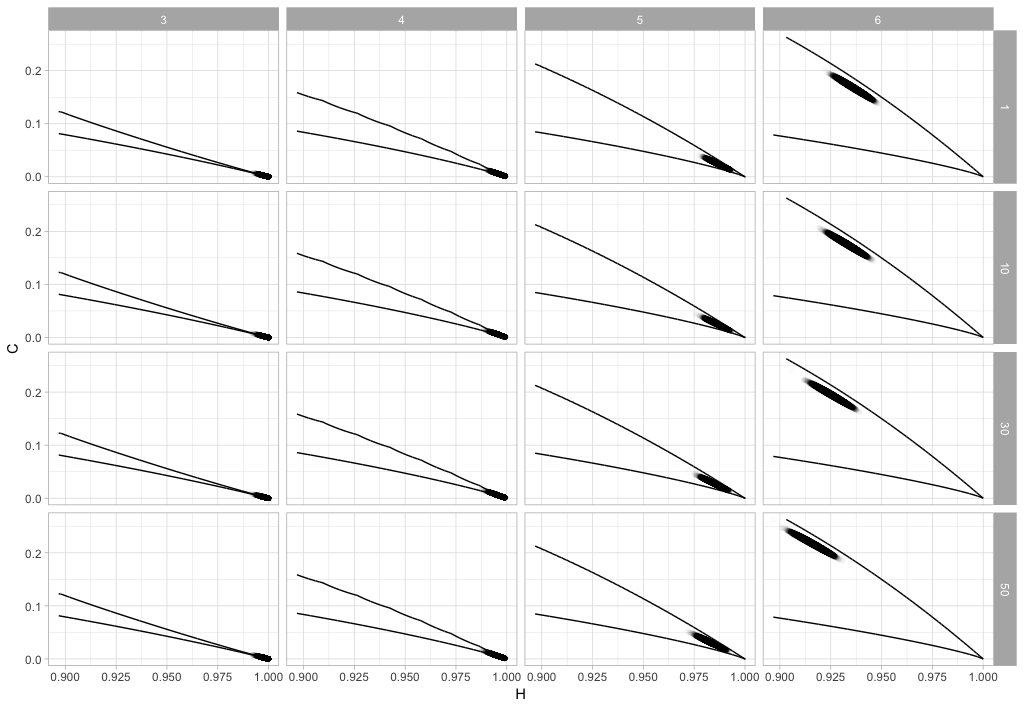
\includegraphics[width=\linewidth]{ScatterAll_Quant_1k}
	\caption{Diagramas de dispersão das sequências quânticas com $1.000$ observações para $D\in\{3, 4, 5, 6\}$ (colunas) e $\tau\in\{1, 10, 30, 50\}$ (linhas), com curvas de complexidade mínima e máxima no plano Entropia-Complexidade.}\label{Fig:ScatterAll_Quant_1k}
\end{figure}

\begin{figure}[hbt]
	\centering
	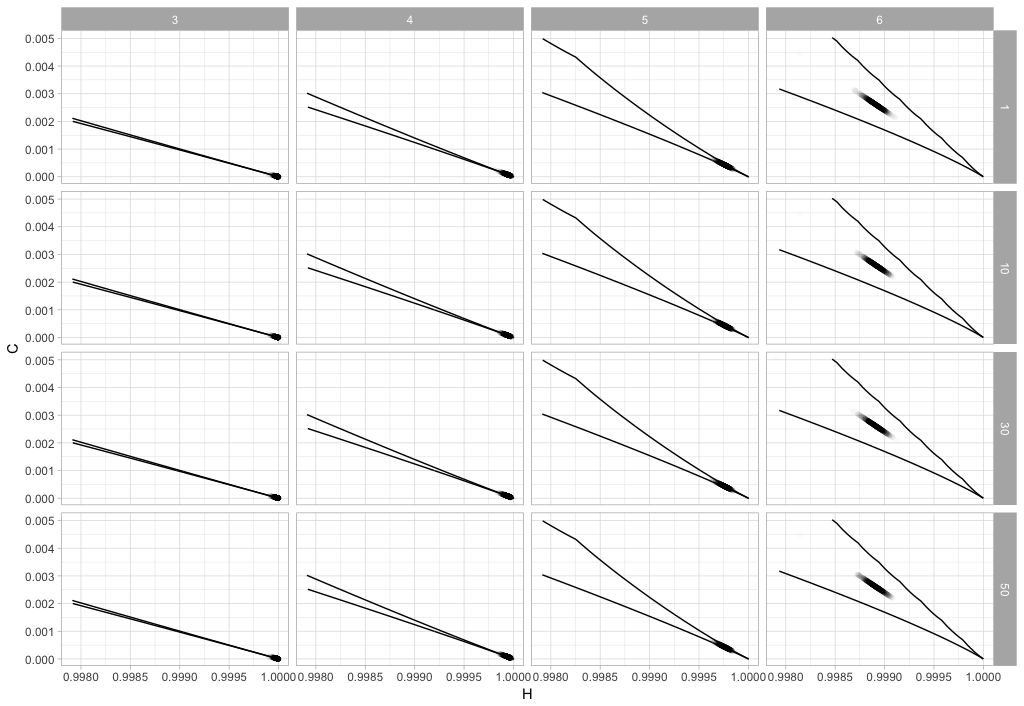
\includegraphics[width=\linewidth]{ScatterAll_Quant_50k}
	\caption{Diagramas de dispersão das sequências quânticas com $50.000$ observações para $D\in\{3, 4, 5, 6\}$ (colunas) e $\tau\in\{1, 10, 30, 50\}$ (linhas), com curvas de complexidade mínima e máxima no plano Entropia-Complexidade.}\label{Fig:ScatterAll_Quant_50k}
\end{figure}

As figuras~\ref{Fig:ScatterAll_Radio_1k} e~\ref{Fig:ScatterAll_Radio_50k} mostram os planos Entropia-Complexidade com as respectivas curvas de complexidade mínima e máxima para cada par $D\in\{3, 4, 5, 6\}$ (colunas) e $\tau\in\{1, 10, 30, 50\}$ (linhas), com os \num{52429} pontos observados a partir das sequências obtidas pelo gerador de rádio tomando $1.000$ e $50.000$ sequências respectivamente.


\begin{figure}[hbt]
	\centering
	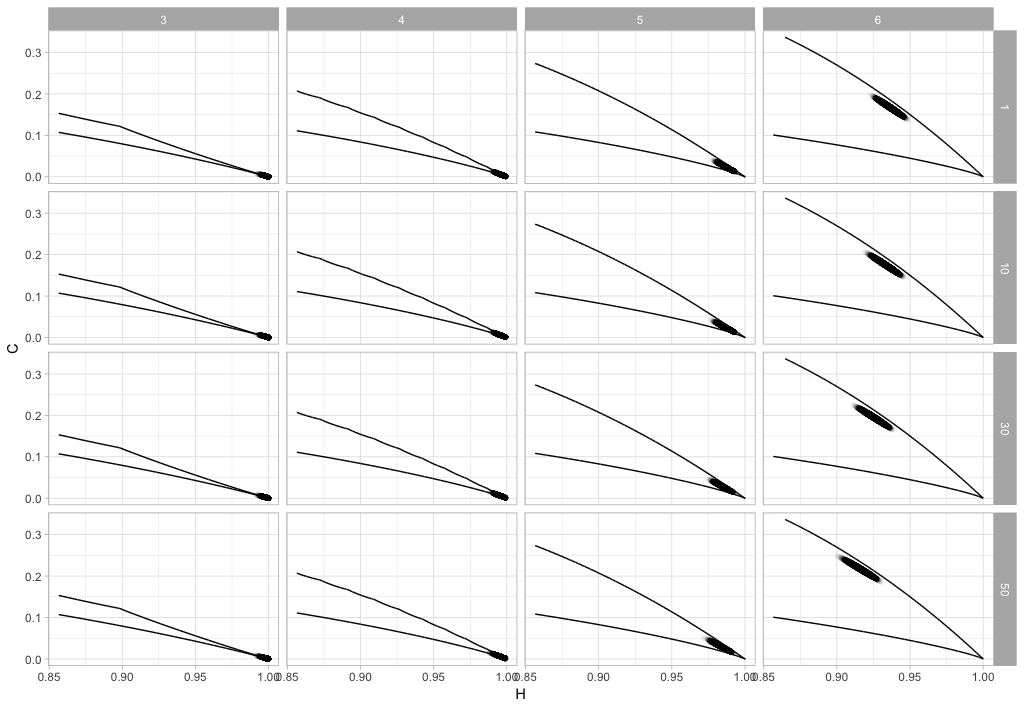
\includegraphics[width=\linewidth]{ScatterAll_Radio_1k}
	\caption{Diagramas de dispersão das sequências de rádio com $1.000$ observações para $D\in\{3, 4, 5, 6\}$ (colunas) e $\tau\in\{1, 10, 30, 50\}$ (linhas), com curvas de complexidade mínima e máxima no plano Entropia-Complexidade.}\label{Fig:ScatterAll_Radio_1k}
\end{figure}

\begin{figure}[hbt]
	\centering
	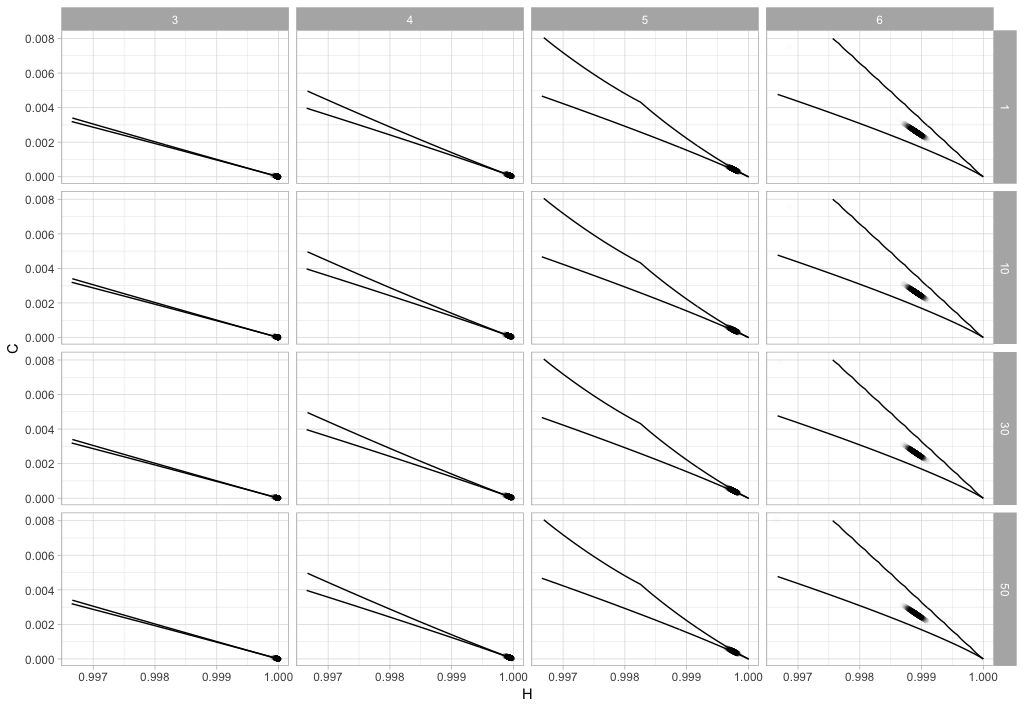
\includegraphics[width=\linewidth]{ScatterAll_Radio_50k}
	\caption{Diagramas de dispersão das sequências de rádio com $50.000$ observações para $D\in\{3, 4, 5, 6\}$ (colunas) e $\tau\in\{1, 10, 30, 50\}$ (linhas), com curvas de complexidade mínima e máxima no plano Entropia-Complexidade.}\label{Fig:ScatterAll_Radio_50k}
\end{figure}

As figuras~\ref{Fig:ScatterAll_MT_1k} e~\ref{Fig:ScatterAll_MT_50k} mostram os planos Entropia-Complexidade com as respectivas curvas de complexidade mínima e máxima para cada par $D\in\{3, 4, 5, 6\}$ (colunas) e $\tau\in\{1, 10, 30, 50\}$ (linhas), com os \num{52429} pontos observados a partir das sequências obtidas pelo gerador Mersenne-Twister tomando $1.000$ e $50.000$ sequências respectivamente.

\begin{figure}[hbt]
	\centering
	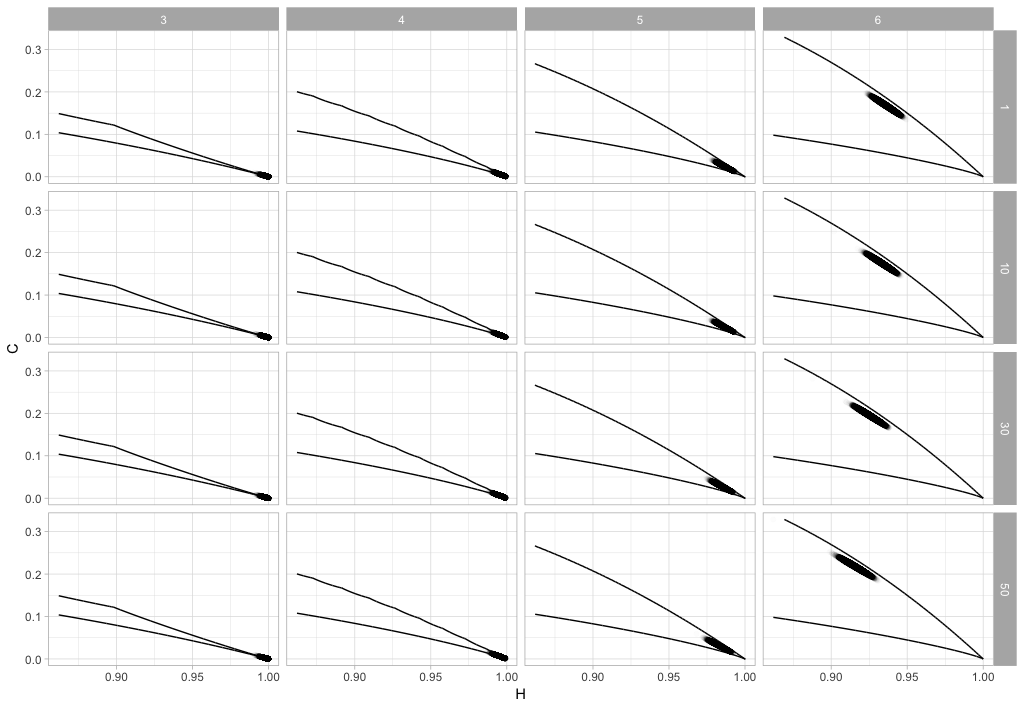
\includegraphics[width=\linewidth]{ScatterAll_MT_1k}
	\caption{Diagramas de dispersão das sequências de Mersenne-Twister com $1.000$ observações para $D\in\{3, 4, 5, 6\}$ (colunas) e $\tau\in\{1, 10, 30, 50\}$ (linhas), com curvas de complexidade mínima e máxima no plano Entropia-Complexidade.}\label{Fig:ScatterAll_MT_1k}
\end{figure}

\begin{figure}[hbt]
	\centering
	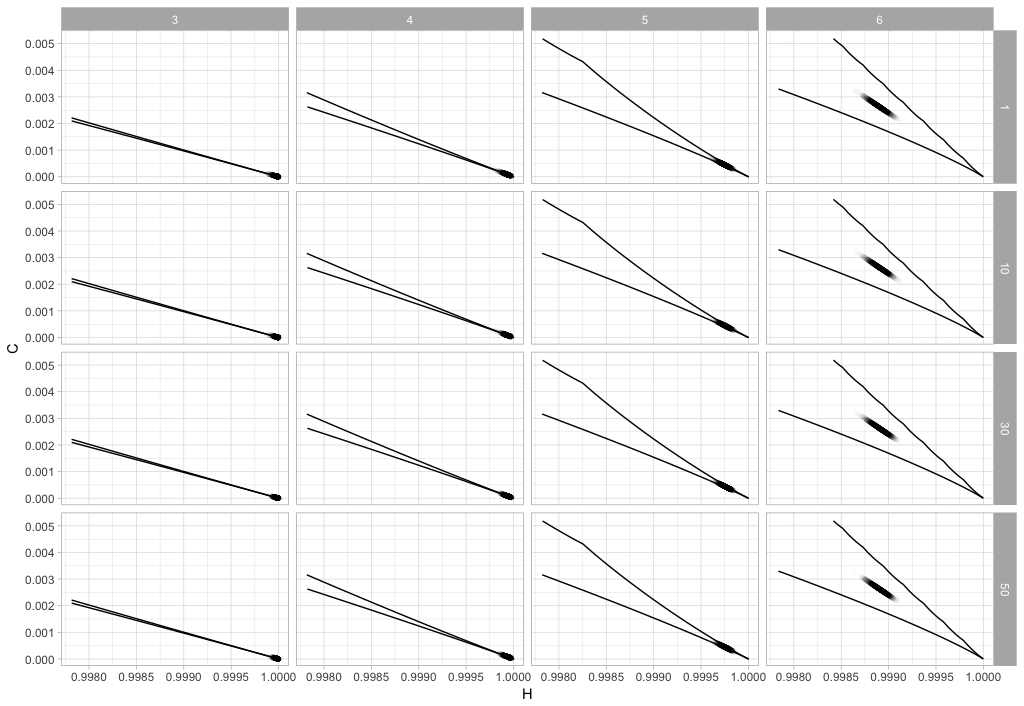
\includegraphics[width=\linewidth]{ScatterAll_MT_50k}
	\caption{Diagramas de dispersão das sequências de Mersenne-Twister com $50.000$ observações para $D\in\{3,4,5,6\}$ (colunas) e $\tau\in\{1,10,30,50\}$ (linhas), com curvas de complexidade mínima e máxima no plano Entropia-Complexidade.}\label{Fig:ScatterAll_MT_50k}
\end{figure}

A olho nu, $D$ é um fator relevante pois os diagramas de dispersão mostram comportamentos que merecem uma análise mais aprofundada, por outro lado não temos certeza de como $\tau$ e o gerador influenciam os resultados. 

As figuras~\ref{fig:GeradorIrrelevante1k} e~\ref{fig:GeradorIrrelevante50k} mostram os histogramas suavizados das distâncias para sequências de tamanho ($N=1.000$, $50.000$) respectivamente, com palavras de tamanho $D=6$  e valores de \textit{lag} ($\tau=1, 50$), sobrepondo os três geradores.
Os gráficos sugerem que o gerador é um fator irrelevante para a distribuição da distância.
Mais adiante veremos que esta impressão não se confirma totalmente.

\begin{figure} %D=6 %N 1000 t1 t 50
	\centering
		\subfigure[$D=6, \tau=1$]{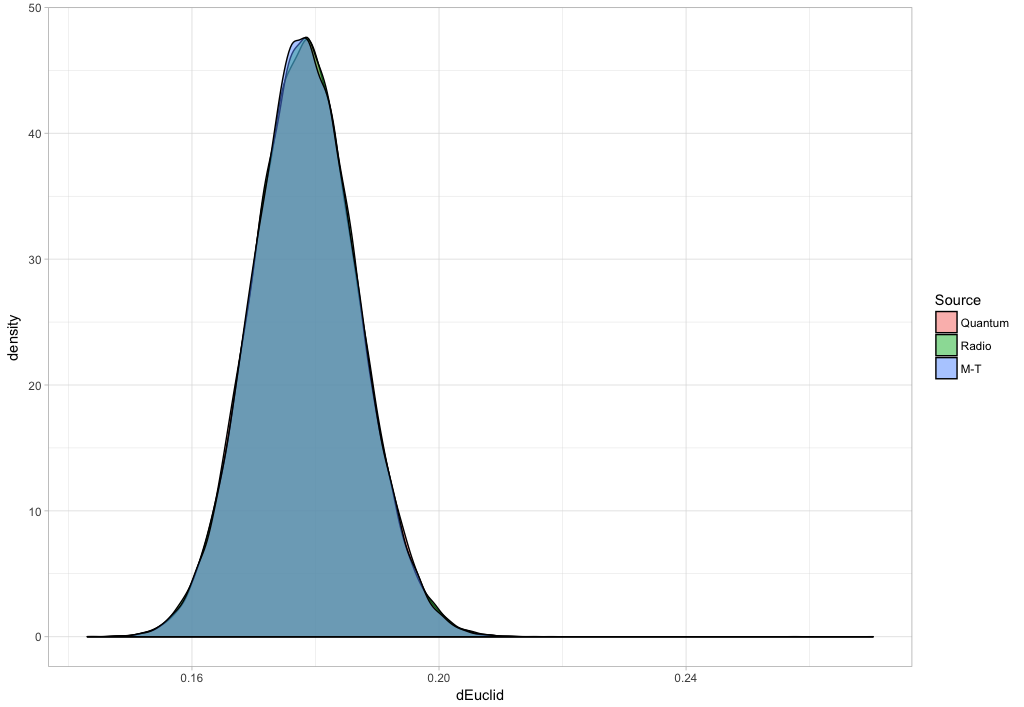
\includegraphics[width=.48\linewidth]{Hist_D6_1k_t1}}
		\subfigure[$D=6, \tau=50$]{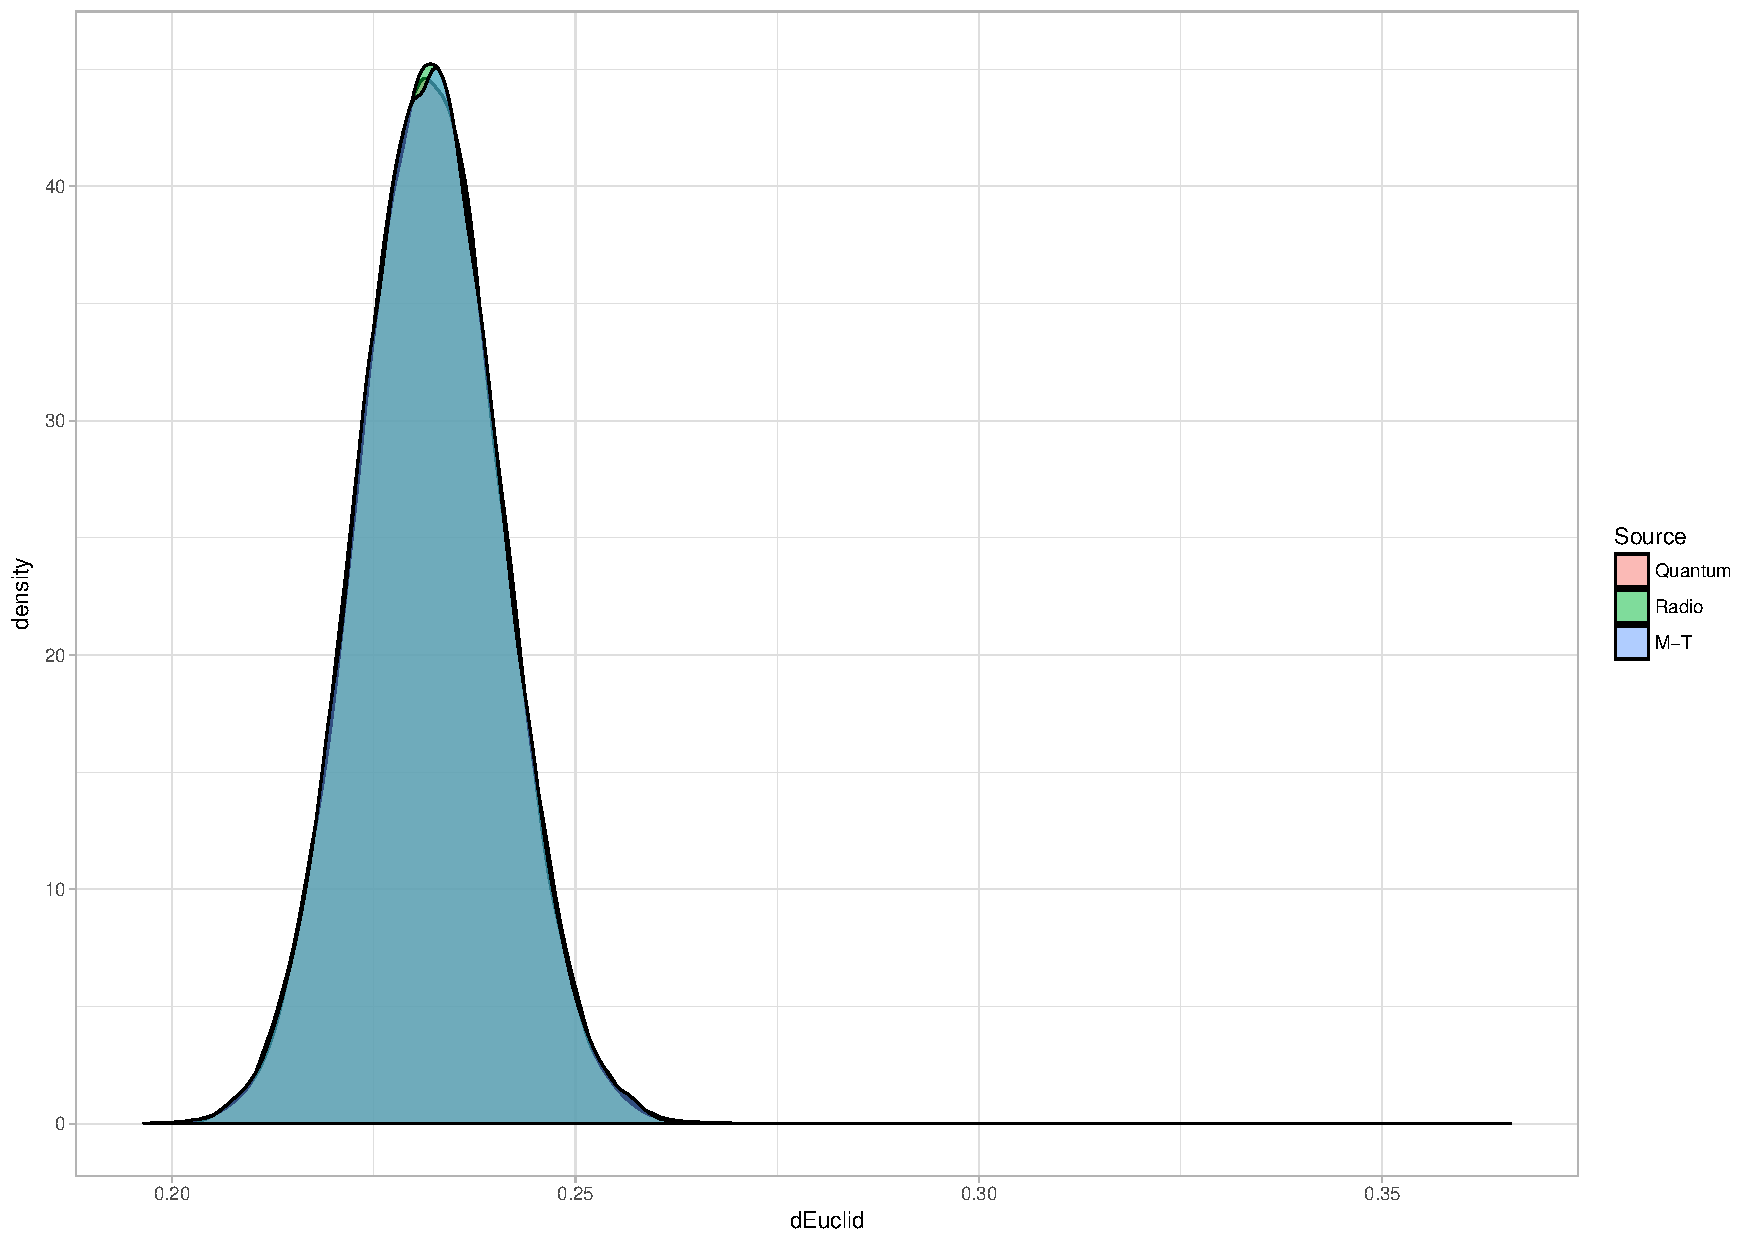
\includegraphics[width=.48\linewidth]{Hist_D6_1k_t50}}
		\caption{Histogramas suavizados de situações que sugerem que o gerador é um fator irrelevante para $N=1.000$}\label{fig:GeradorIrrelevante1k}
\end{figure}

\begin{figure} %D=6 %N 50000 t1 t 50
	\centering
		\subfigure[$D=6, \tau=1$]{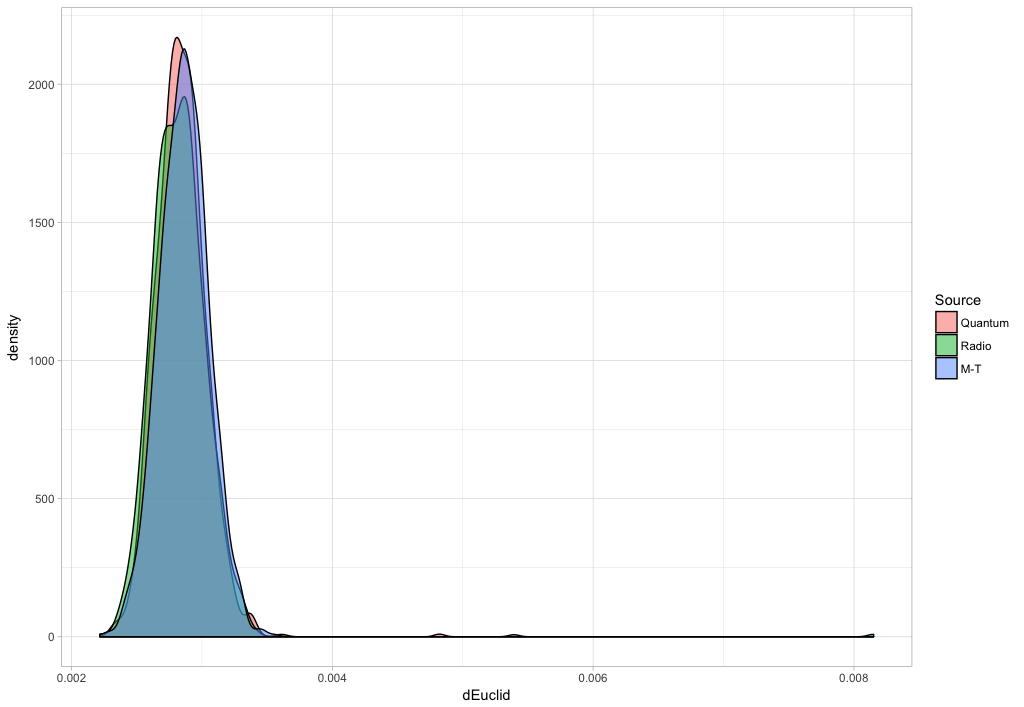
\includegraphics[width=.48\linewidth]{Hist_D6_50k_t1}}
		\subfigure[$D=6, \tau=50$]{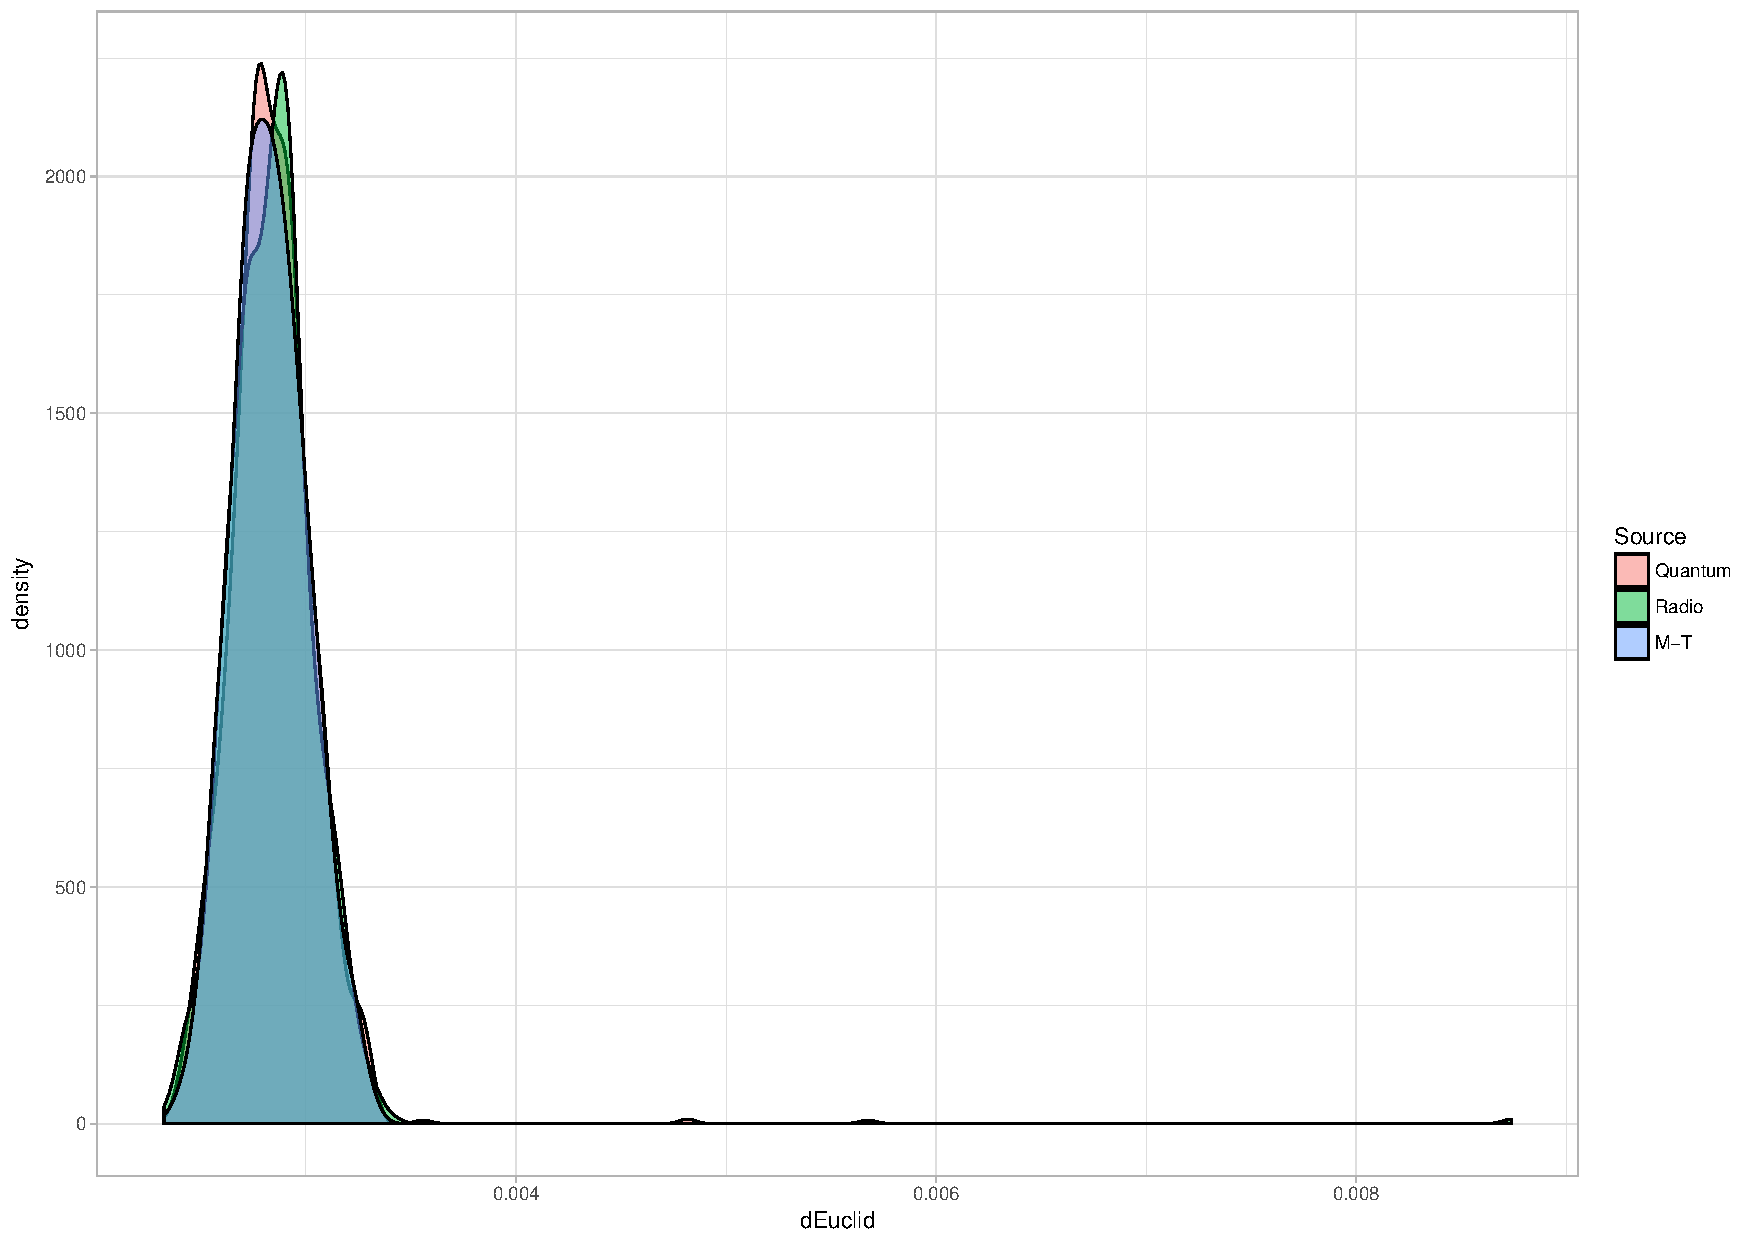
\includegraphics[width=.48\linewidth]{Hist_D6_50k_t50}}
		\caption{Histogramas suavizados de situações que sugerem que o gerador é um fator irrelevante também para $N=50.000$}\label{fig:GeradorIrrelevante50k}
\end{figure}

A figura~\ref{fig:NRelevante} mostra os histogramas suavizados das distâncias dos três geradores para palavras de tamanho $D=6$ e dois valores de \textit{lag} ($\tau=1$, $50$), sobrepondo os resultados obtidos com os dois tamanhos de sequências ($N=1.000$, $50.000$).
Os gráficos sugerem fortemente que o tamanho das sequências é um fator relevante para a distribuição da distância.

\begin{figure} %D=6 %t 1 N 1000 N 50000 (três geradores) %t 50 N 1000 N 50000 (três geradores)
	\centering
		\subfigure[$D=6$, $\tau=1$]{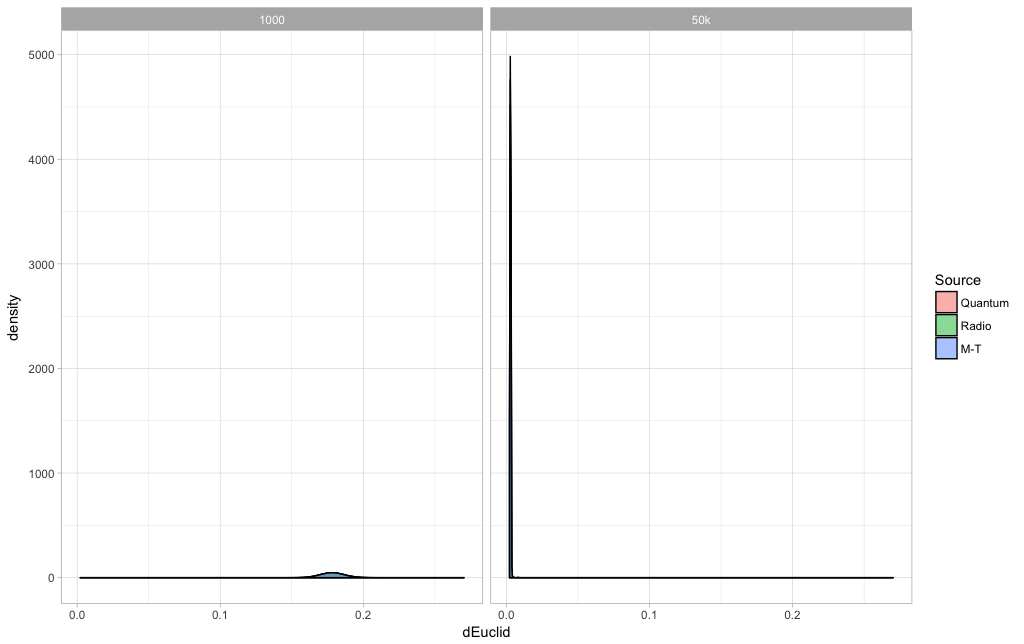
\includegraphics[width=.48\linewidth]{Hist_D6_t1}}
		\subfigure[$D=6$, $\tau=50$]{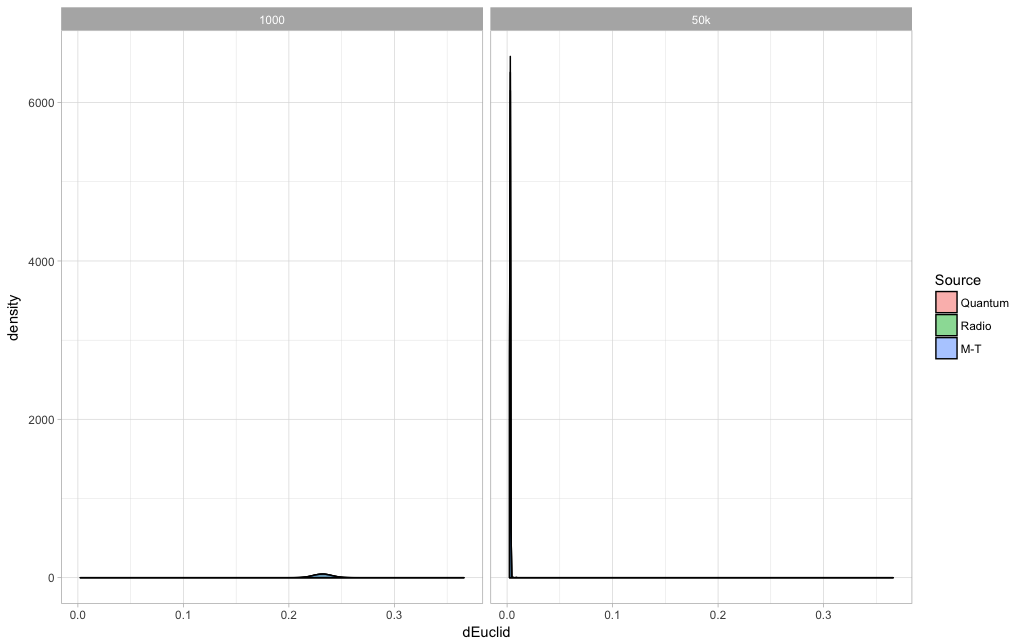
\includegraphics[width=.48\linewidth]{Hist_D6_t50}}
	\caption{Histogramas suavizados de situações que sugerem que o $N$ é um fator relevante}\label{fig:NRelevante}
\end{figure}

A figura~\ref{fig:DRelevante} mostra os histogramas suavizados das distâncias dos três geradores para dois tamanhos de sequências ($N=1.000$, $50.000$) e dois valores de \textit{lag} ($\tau=1$, $50$), sobrepondo os resultados obtidos com os diferentes tamanhos de palavras ($D=3$, $4$, $5$, $6$).
Os gráficos sugerem fortemente que o tamanho das palavras é um fator relevante para a distribuição da distância.

\begin{figure} %t 1 N 1000, D 3 D 4 D 5 D 6 %t 50 N 50000, D 3 D 4 D 5 D 6
	\centering
		\subfigure[$\tau=1$, $D=1.000$]{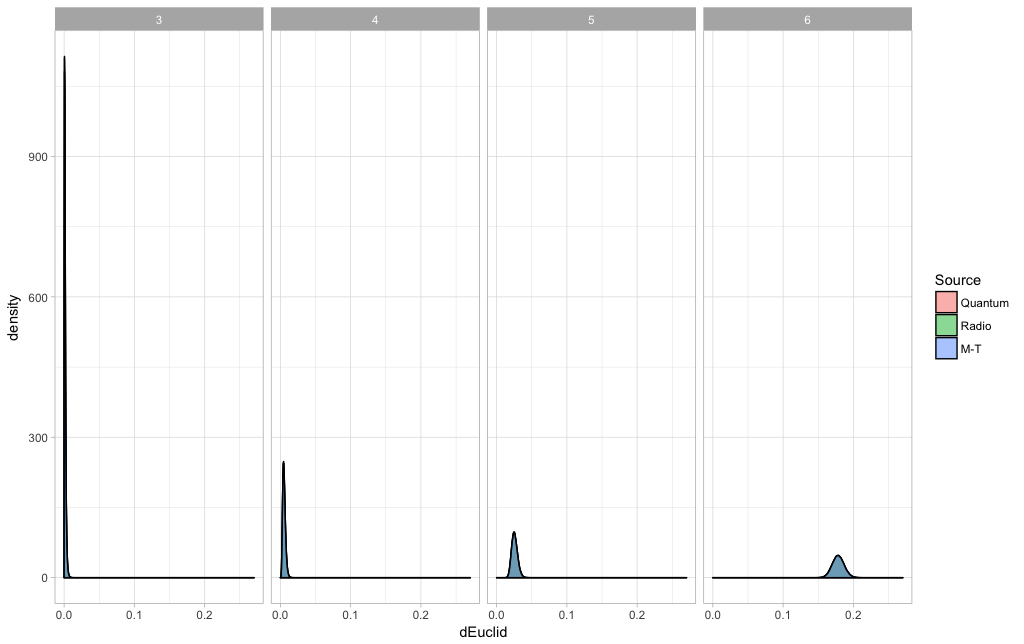
\includegraphics[width=.48\linewidth]{Hist_t1_1k}}
		\subfigure[$D=6$, $\tau=50$]{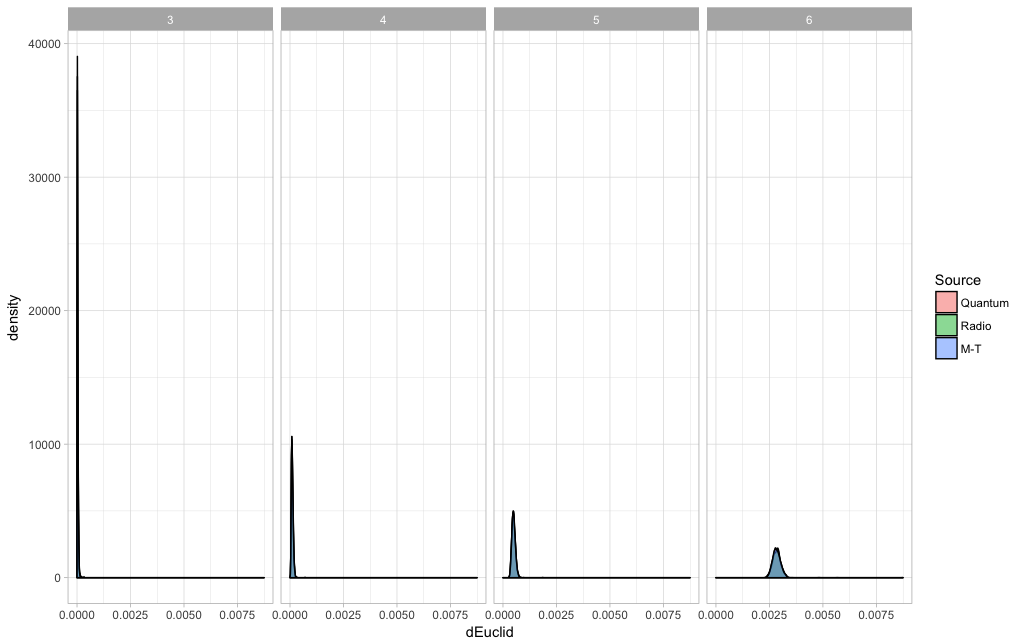
\includegraphics[width=.48\linewidth]{Hist_t50_50k}}
	\caption{Histogramas suavizados de situações que sugerem que o $D$ é um fator relevante}\label{fig:DRelevante}
\end{figure}



\begin{figure} %D 6 %N 1000, t 1 t 10 t 30 t 50 %N 50000, t 1 t 10 t 30 t 50
	\centering
	\subfigure[$\tau=1$, $D=1.000$]{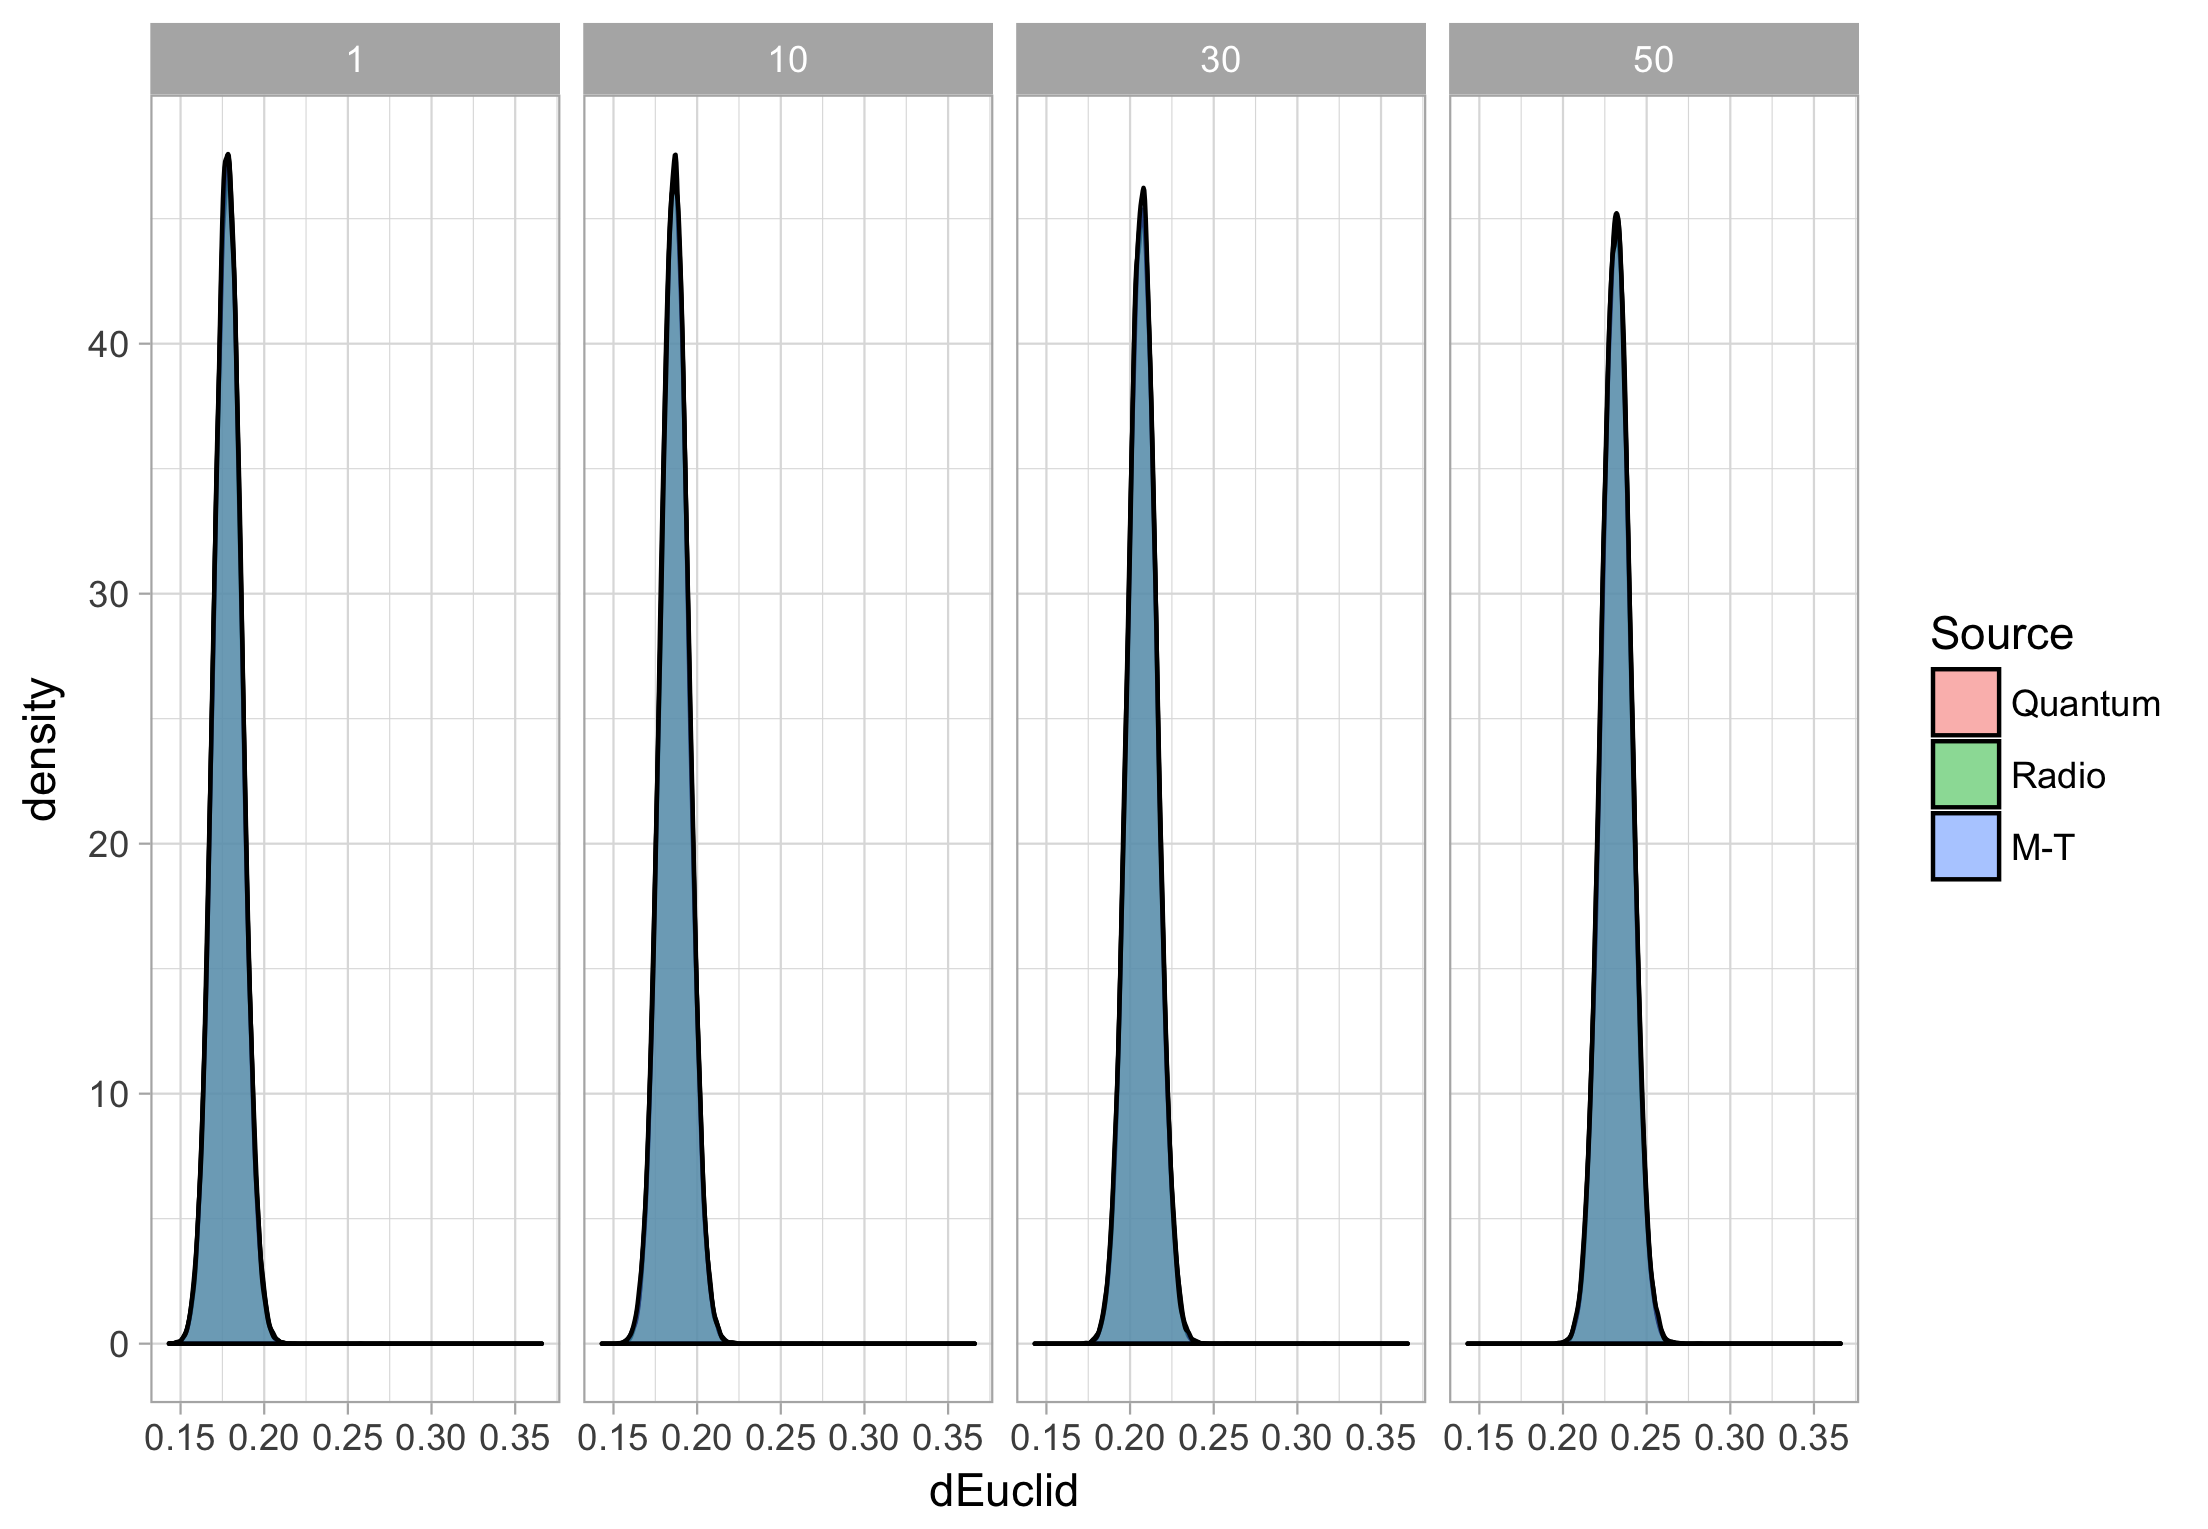
\includegraphics[width=.48\linewidth]{Hist_D6_1k}}
	\subfigure[$D=6$, $\tau=50$]{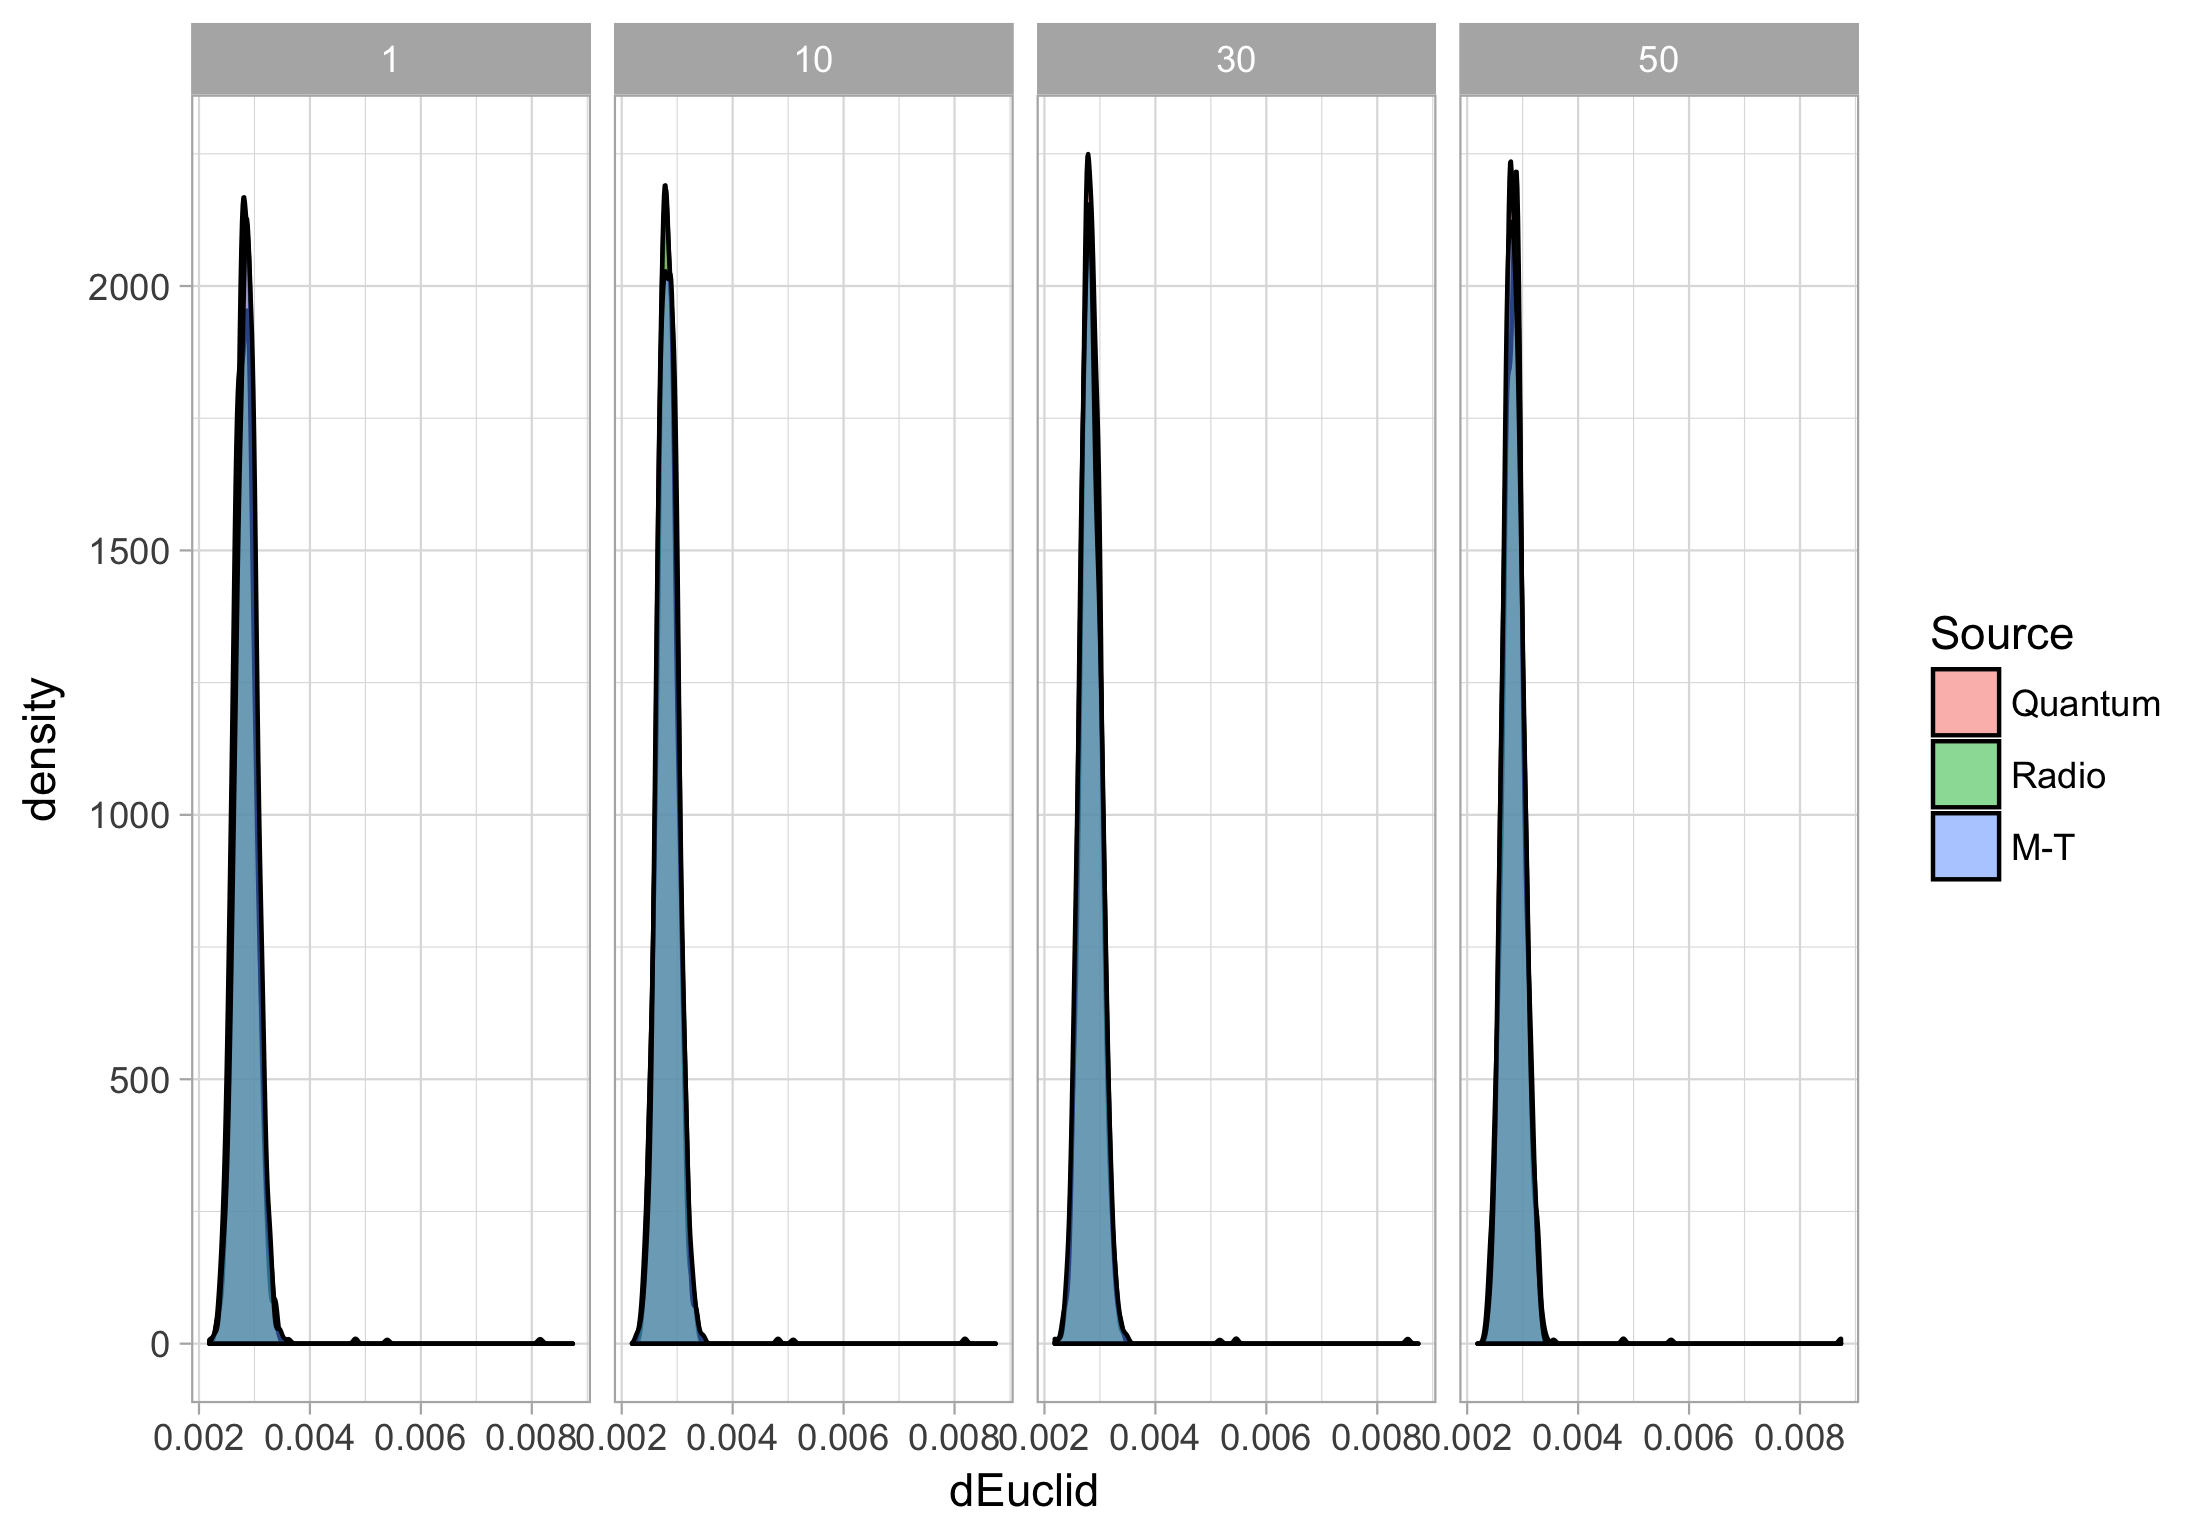
\includegraphics[width=.48\linewidth]{Hist_D6_50k}}
\caption{Histogramas suavizados de situações que sugerem que o $\tau$ é um fator relevante}\label{fig:tRelevante}
\end{figure}

Para consolidar esta análise realizamos a seguir testes Kolmogorov-Smirnov afim de analisar a influência dos fatores envolvidos nesta análise.

A Tabela~\ref{tab:KS_1000} mostra os $p$-valores dos testes de Kolmogorov-Smirnov aplicados a pares de distâncias calculadas sobre sequências de tamanho $1000$, variando $D$ e $\tau$.
Verificamos que há excelente aderência entre os pares de distâncias de sequências Quânticas e de Rádio.
Já quando a comparação é feita com distâncias de sequências de Mersenne-Twister (M-T), a aderência diminui um pouco.

\begin{table}[hbt]
	\centering
	\caption{Teste de Kolmogorov-Smirnov aplicado a pares de sequências para $1.000$ observações.}\label{tab:KS_1000}
	\begin{tabular}{cccccc}
		\toprule
		Par  &    $D$ & $\tau=1$   &   $\tau=10$   &   $\tau=30$   &   $\tau=50$   \\ \midrule
Quântica vs.\ Rádio		& $D=3$ & 0.18034676 & 0.08582490 & 0.58096350 & 0.32626542 \\
		& $D=4$ & 0.21708776 & 0.60690204 & 0.08116764 & 0.46372312  \\
		& $D=5$ & 0.32388371 & 0.53394280 & 0.46970138 & 0.02768674  \\
		& $D=6$ & 0.61501858 & 0.63403661 & 0.54795745 & 0.15353799  \\ \midrule
Quântica vs. M-T & $D=3$ & 0.09400120 & 0.22995096 & 0.36766759 &  0.03706359 \\
		& $D=4$ & 0.25188769 & 0.35844686 & 0.16768952 &  0.18237754 \\
		& $D=5$ & 0.97552039 & 0.79878301 & 0.12852918 &  0.08764347 \\
		& $D=6$ & 0.47615384 & 0.42420007 & 0.55290011 &  0.79669144 \\ \midrule
Rádio vs.\ M-T & $D=3$ & 0.008560614 & 0.496450214 & 0.982419336 & 0.390237891 \\
		& $D=4$ & 0.003804157 & 0.229503619 & 0.629158543 & 0.651783589 \\
		& $D=5$ & 0.254216237 & 0.179697451 & 0.824743440 & 0.071709252 \\
		& $D=6$ & 0.846441994 & 0.033726860 & 0.493286733 & 0.184856861 \\
		\bottomrule
	\end{tabular}
\end{table}

Os $p$-valores reportados para distâncias obtidas com sequências de tamanho $N=1000$ não permitem concluir que haja diferenças significativas.
Essa constatação será revertida ao analisar distâncias entre sequências de tamanho $N=50000$.

A Tabela~\ref{tab:KS_50k} mostra os $p$-valores dos testes de Kolmogorov-Smirnov aplicados a pares de distâncias calculadas sobre sequências de tamanho $50000$, variando $D$ e $\tau$.
Verificamos que há excelente aderência entre os pares de distâncias de sequências Quânticas e de Rádio.
Já quando a comparação é feita com distâncias de sequências de Mersenne-Twister (M-T), a aderência diminui de forma sistemática e significativa para $\tau=1$.

\begin{table}[hbt]
	\centering
	\caption{Teste de Kolmogorov-Smirnov aplicado a pares de sequências para $50.000$ observações.}\label{tab:KS_50k}
	\begin{tabular}{cccccc}
		\toprule
		Par  & $D$ &   $\tau=1$   &   $\tau=10$   &   $\tau=30$   &   $\tau=50$   \\ \midrule
Quântica vs.\ Rádio		& $D=3$ & 0.13862662 & 0.93677447 & 0.07714702 &  0.46405291 \\
		& $D=4$ & 0.68079537 & 0.90035466 & 0.60801914 &  0.77908261 \\
		& $D=5$ & 0.14371256 & 0.76662067 & 0.64456996 &  0.91315843 \\
		& $D=6$ & 0.02268670 & 0.49307044 & 0.53135926 &  0.30074267 \\ \midrule
Quântica vs.\ M-T & $D=3$ & 6.074571e-10 & 1.388898e-01 & 2.682058e-01 & 4.822849e-01 \\
		& $D=4$ & 6.592620e-09 & 2.987721e-02 & 8.438134e-01 & 7.923220e-01 \\
		& $D=5$ & 9.424114e-08 & 3.289299e-02 & 7.681676e-01 & 8.405168e-01 \\
		& $D=6$ & 9.058821e-04 & 7.075225e-01 & 2.982731e-01 & 3.614763e-01 \\ \midrule
Rádio vs.\ M-T		& $D=3$ & 1.226271e-09 & 1.609665e-01 & 1.465970e-01 & 1.914937e-01 \\
		& $D=4$ & 2.190462e-10 & 1.277762e-02 & 2.069821e-01 & 9.963221e-01 \\
		& $D=5$ & 1.438372e-11 & 1.267622e-02 & 4.364935e-01 & 9.999998e-01 \\
		& $D=6$ & 3.749001e-06 & 2.263466e-01 & 7.419248e-01 & 4.014641e-01 \\
		\bottomrule
	\end{tabular}
\end{table}

Os $p$-valores observados na Tabela~\ref{tab:KS_50k} nos levam a concluir que não é possível desconsiderar a fonte de dados como um fator relevante quando se trata do gerador de Mersenne-Twister.
Já as distâncias das sequências produzidas pelos geradores Quântico e de Rádio são indistinguíveis e, portanto, não podemos descartar a hipótese dessas fontes serem idênticas para a medida considerada.

%A figura~\ref{Fig:ScatterAllRandom} mostra os planos Entropia-Complexidade com as respectivas curvas de complexidade mínima e máxima para cada par $D\in\{3,4,5,6\}$ (colunas) e $\tau\in\{1,10,30,50\}$ (linhas), com os \num{52429} pontos observados a partir das sequências obtidas pelo gerador de rádio.
%Os pontos foram desenhados com \SI{1}{\percent} de transparência, para evidenciar as regiões mais e menos densas.
%
%\begin{figure}[hbt]
%	\centering
%	\includegraphics[width=\linewidth]{ScatterAllRandom}
%	\caption{Diagramas de dispersão das sequências de rádio para $D\in\{3,4,5,6\}$ (colunas) e $\tau\in\{1,10,30,50\}$ (linhas), com curvas de complexidade mínima e máxima no plano Entropia-Complexidade.}\label{Fig:ScatterAllRandom}
%\end{figure}
%
%A figura~\ref{Fig:ScatterAllMT} mostra os planos Entropia-Complexidade com as respectivas curvas de complexidade mínima e máxima para cada par $D\in\{3,4,5,6\}$ (colunas) e $\tau\in\{1,10,30,50\}$ (linhas), com os \num{52429} pontos observados a partir das sequências obtidas pelo gerador de Mersenne-Twister.
%Os pontos foram desenhados com \SI{1}{\percent} de transparência, para evidenciar as regiões mais e menos densas.
%
%\begin{figure}[hbt]
%	\centering
%	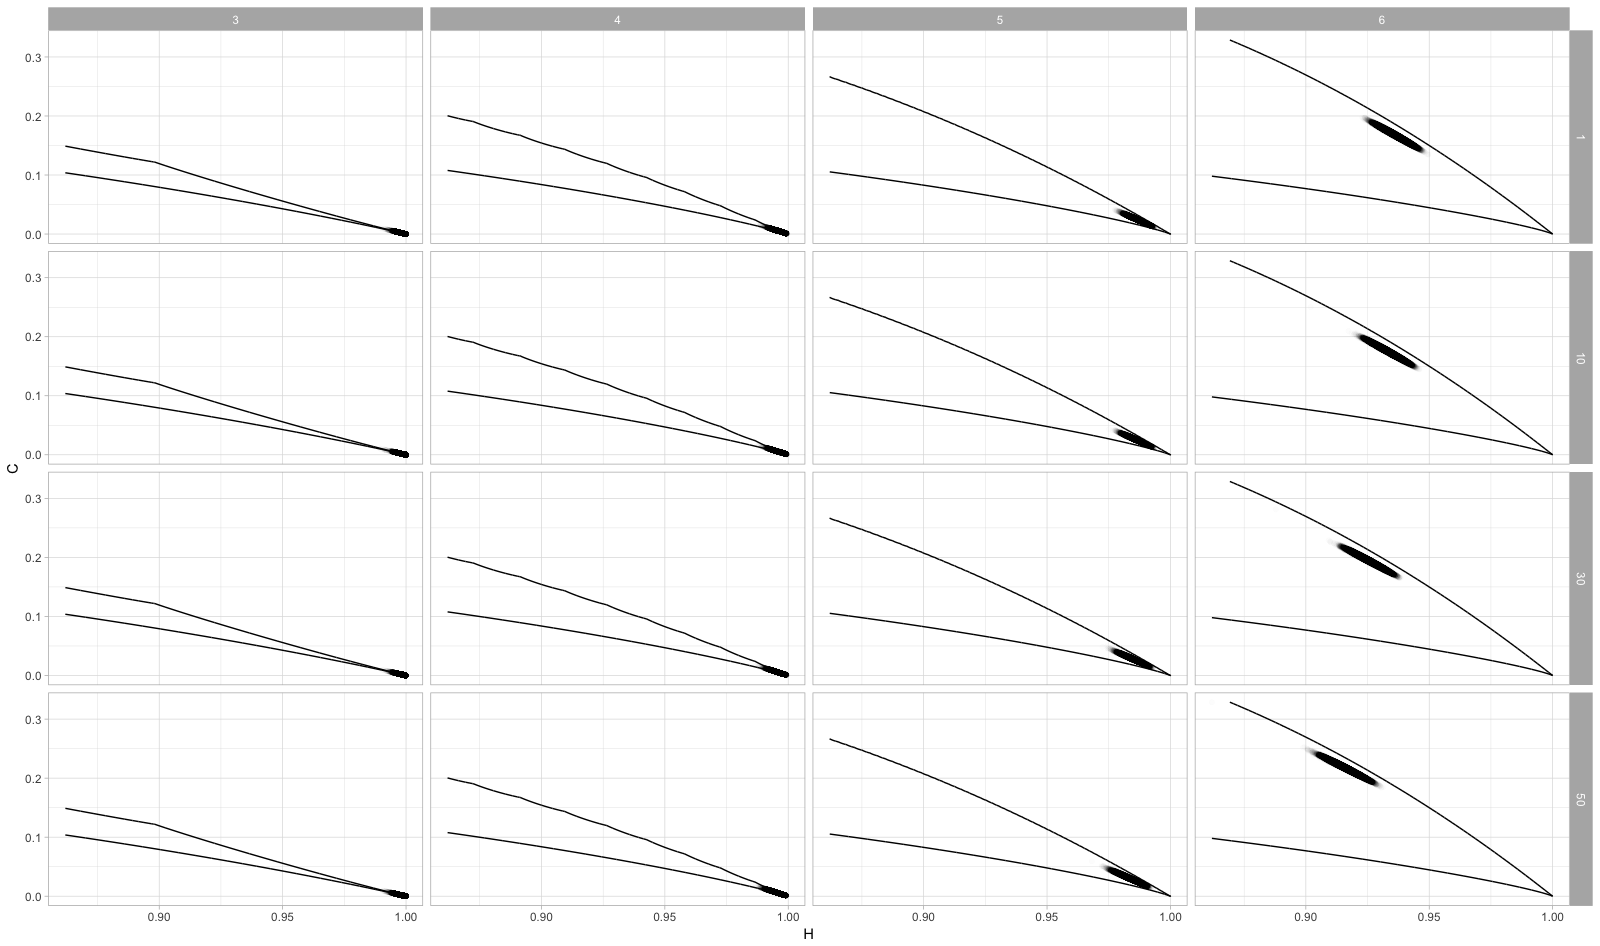
\includegraphics[width=\linewidth]{ScatterAllMT}
%	\caption{Diagramas de dispersão das sequências de Mersenne-Twister para $D\in\{3,4,5,6\}$ (colunas) e $\tau\in\{1,10,30,50\}$ (linhas), com curvas de complexidade mínima e máxima no plano Entropia-Complexidade.}\label{Fig:ScatterAllMT}
%\end{figure}

\begin{figure}[hbt]
\centering
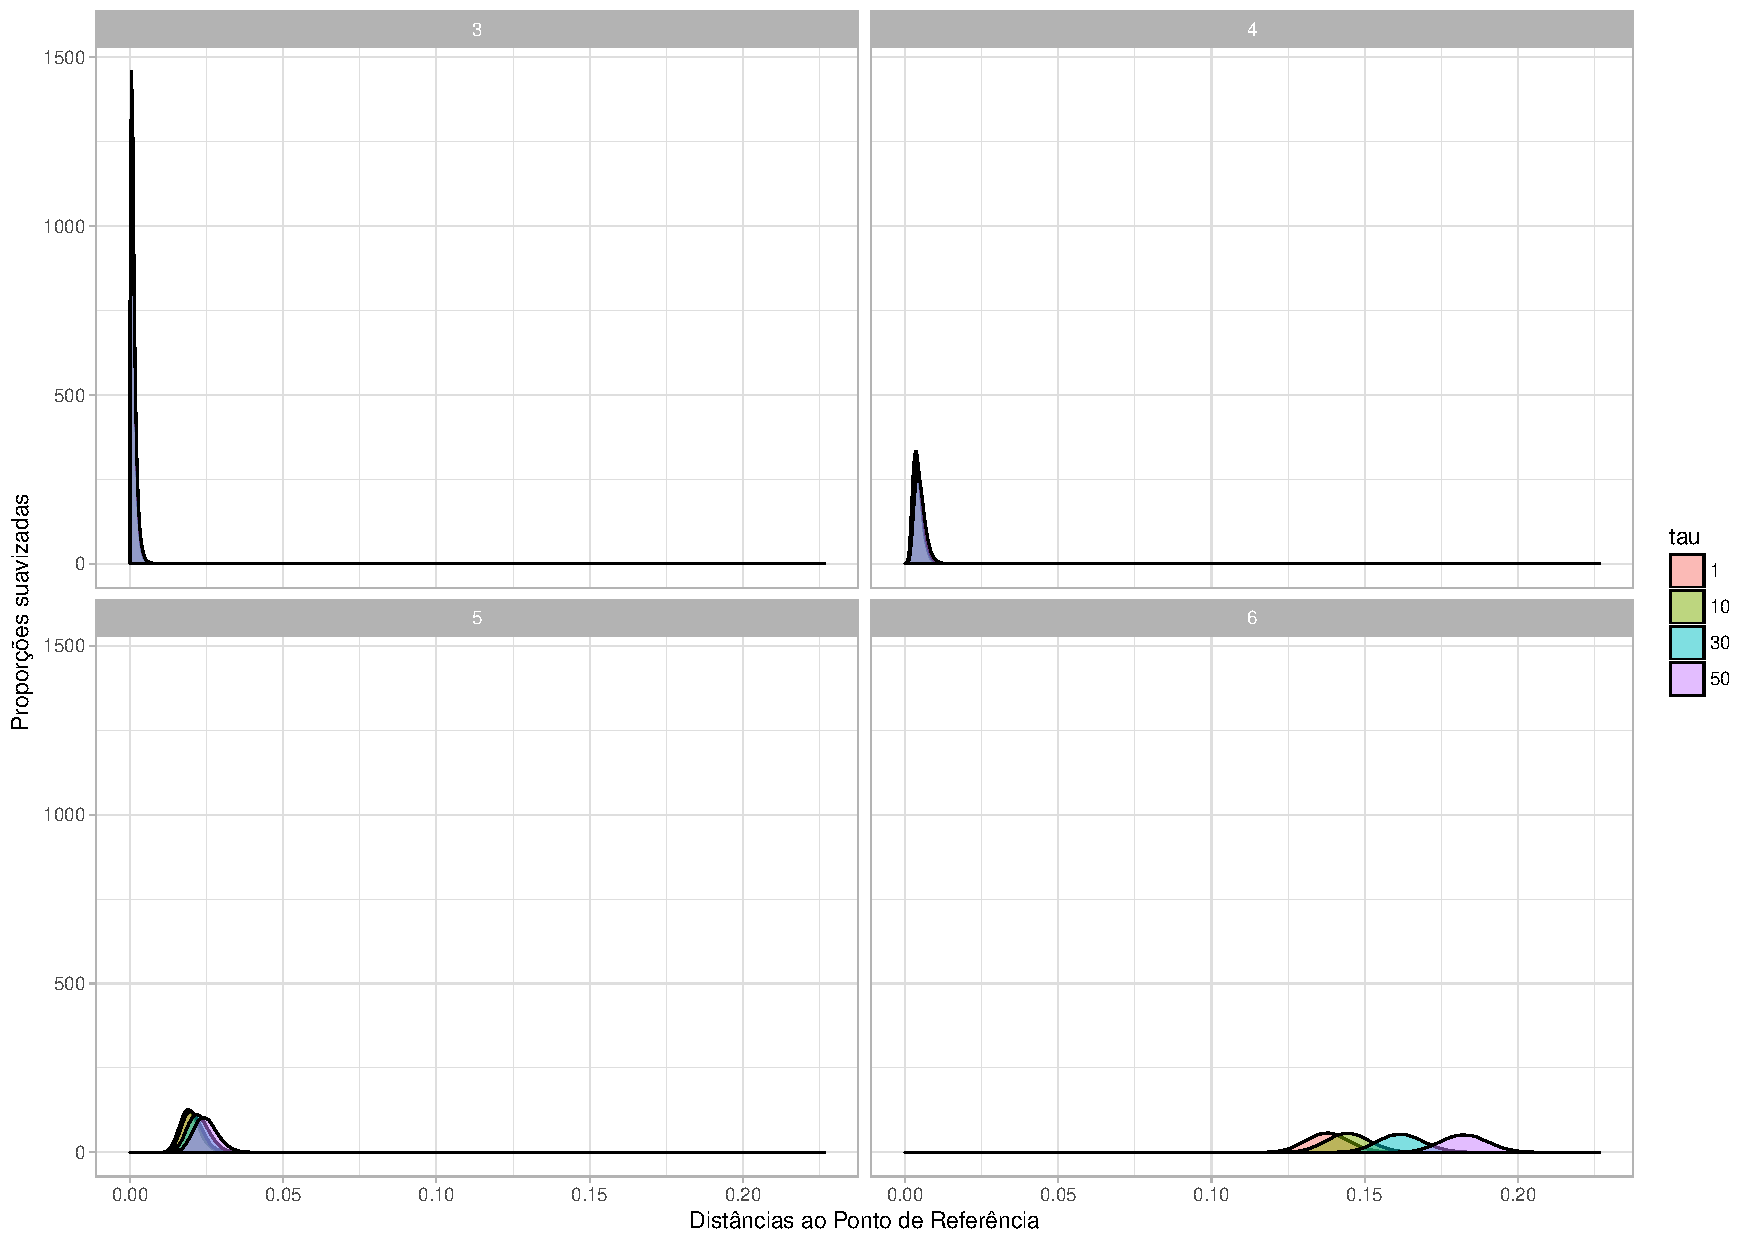
\includegraphics[width=\linewidth]{HistoDistanciasQuantTodas}
\caption{Histogramas suavizados das distâncias euclidianas dos padrões ao ponto de referência, para $D\in\{3,4,5,6\}$ (colunas) e $\tau\in\{1,10,30,50\}$ (linhas).}\label{Fig:HistoDistanciasQuantTodas}
\end{figure}

A figura~\ref{Fig:HistoDistanciasQuantTodas} sugere que o comportamento das distâncias euclidianas ao ponto de referência muda conforme o tamanho do padrão $D$ varia.
Além disso, também são perceptíveis mudanças de comportamento em função do \textit{lag} $\tau$ quando $D=5,6$.

Da análise aqui apresentada concluímos que, à luz da distância do ponto característico de uma sequência ao ponto de referência, os dois geradores físicos produzem sequências indistinguíveis.
Diante disso, nos cálculos subsequentes faremos a junção desses conjuntos de dados, que denominaremos simplesmente ``aleatórios'' no que segue.

Já o gerador de Mersenne-Twister apresenta diferenças em relação aos geradores de origem física.
Por se tratar de um gerador algorítmico e, portanto, pseudoaleatório, ele será tratado como objeto de análise e não como padrão para estabelecer critérios de qualidade.

\section{Análise das sequências aleatórias}

\begin{figure}
\centering
\subfigure[Escala linear\label{Fig:ScatterQuantD3tau1}]{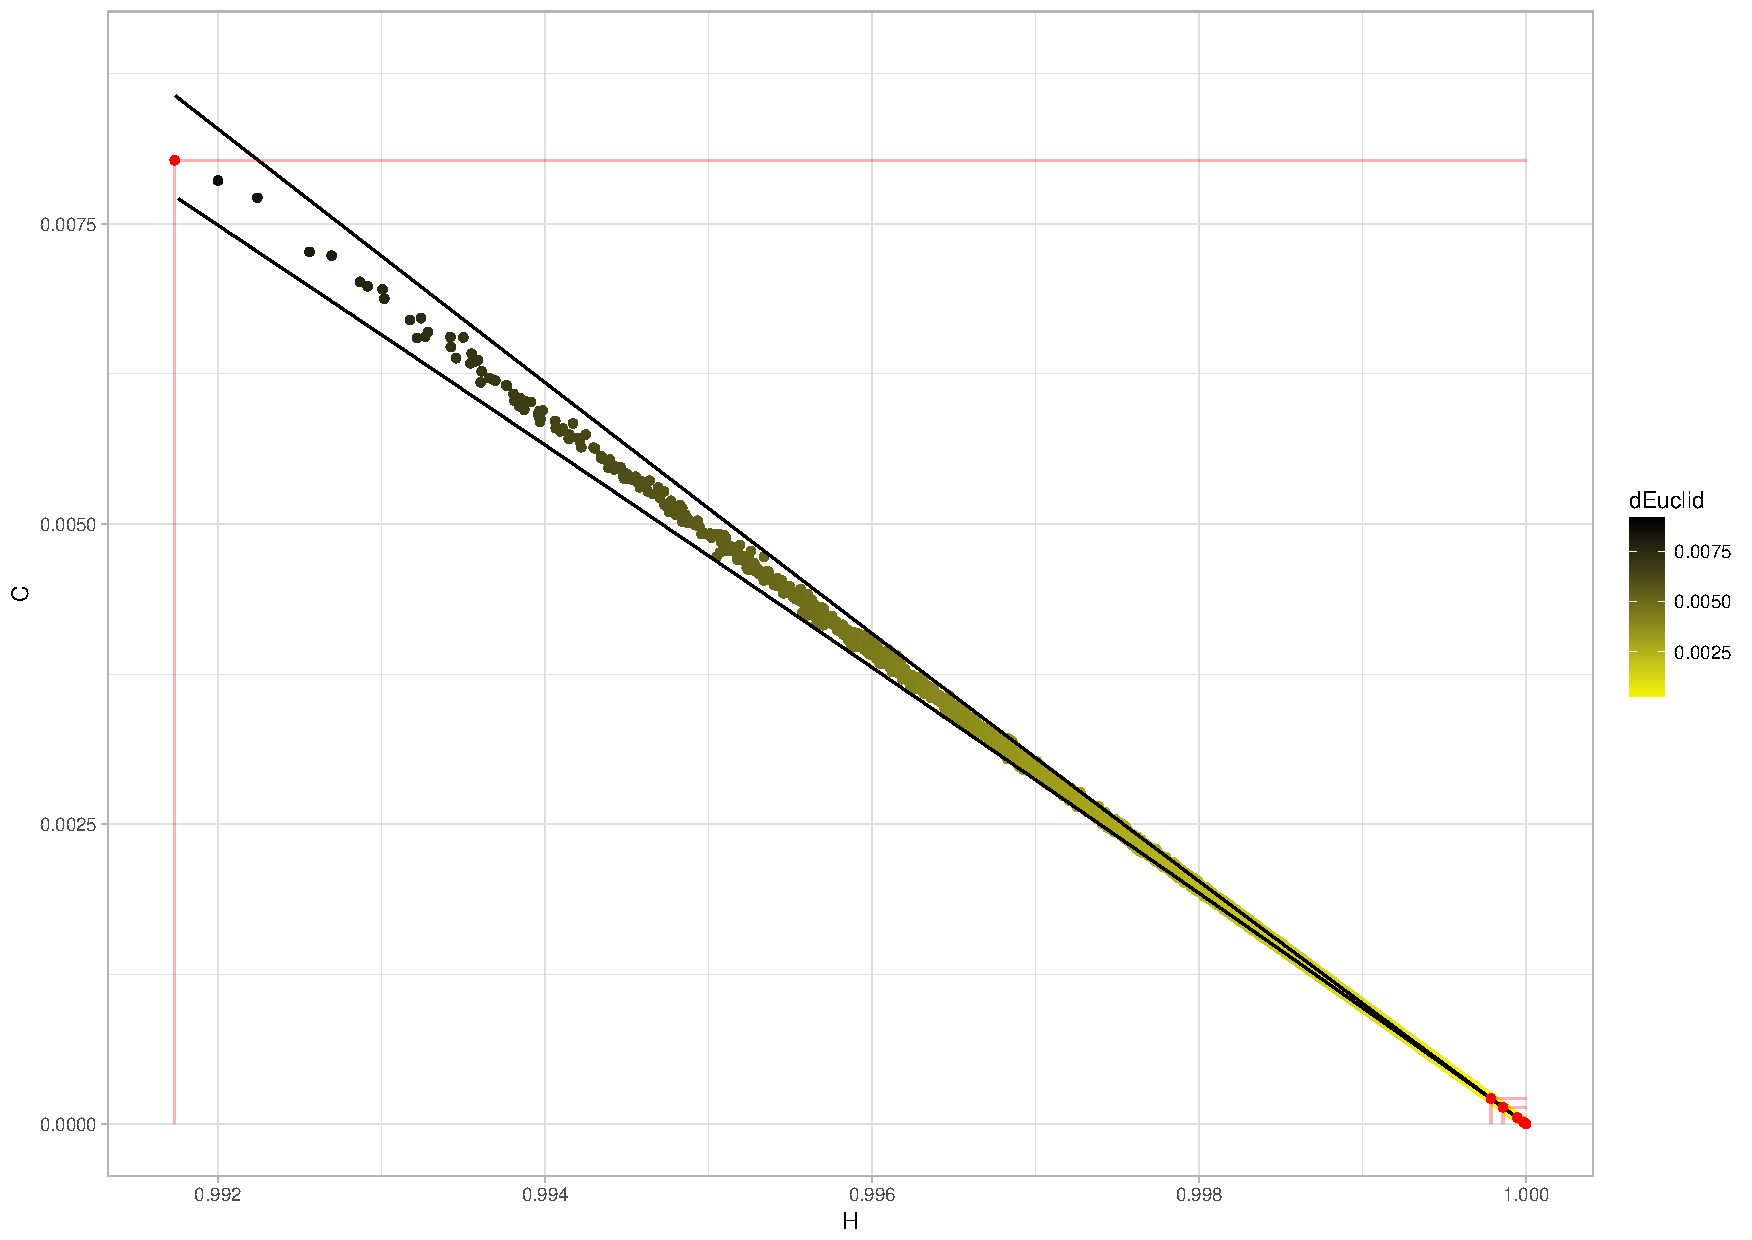
\includegraphics[width=.48\linewidth]{ScatterQuantD3tau1}}
\subfigure[Escala logarítmica\label{Fig:ScatterQuantD3tau1log}]{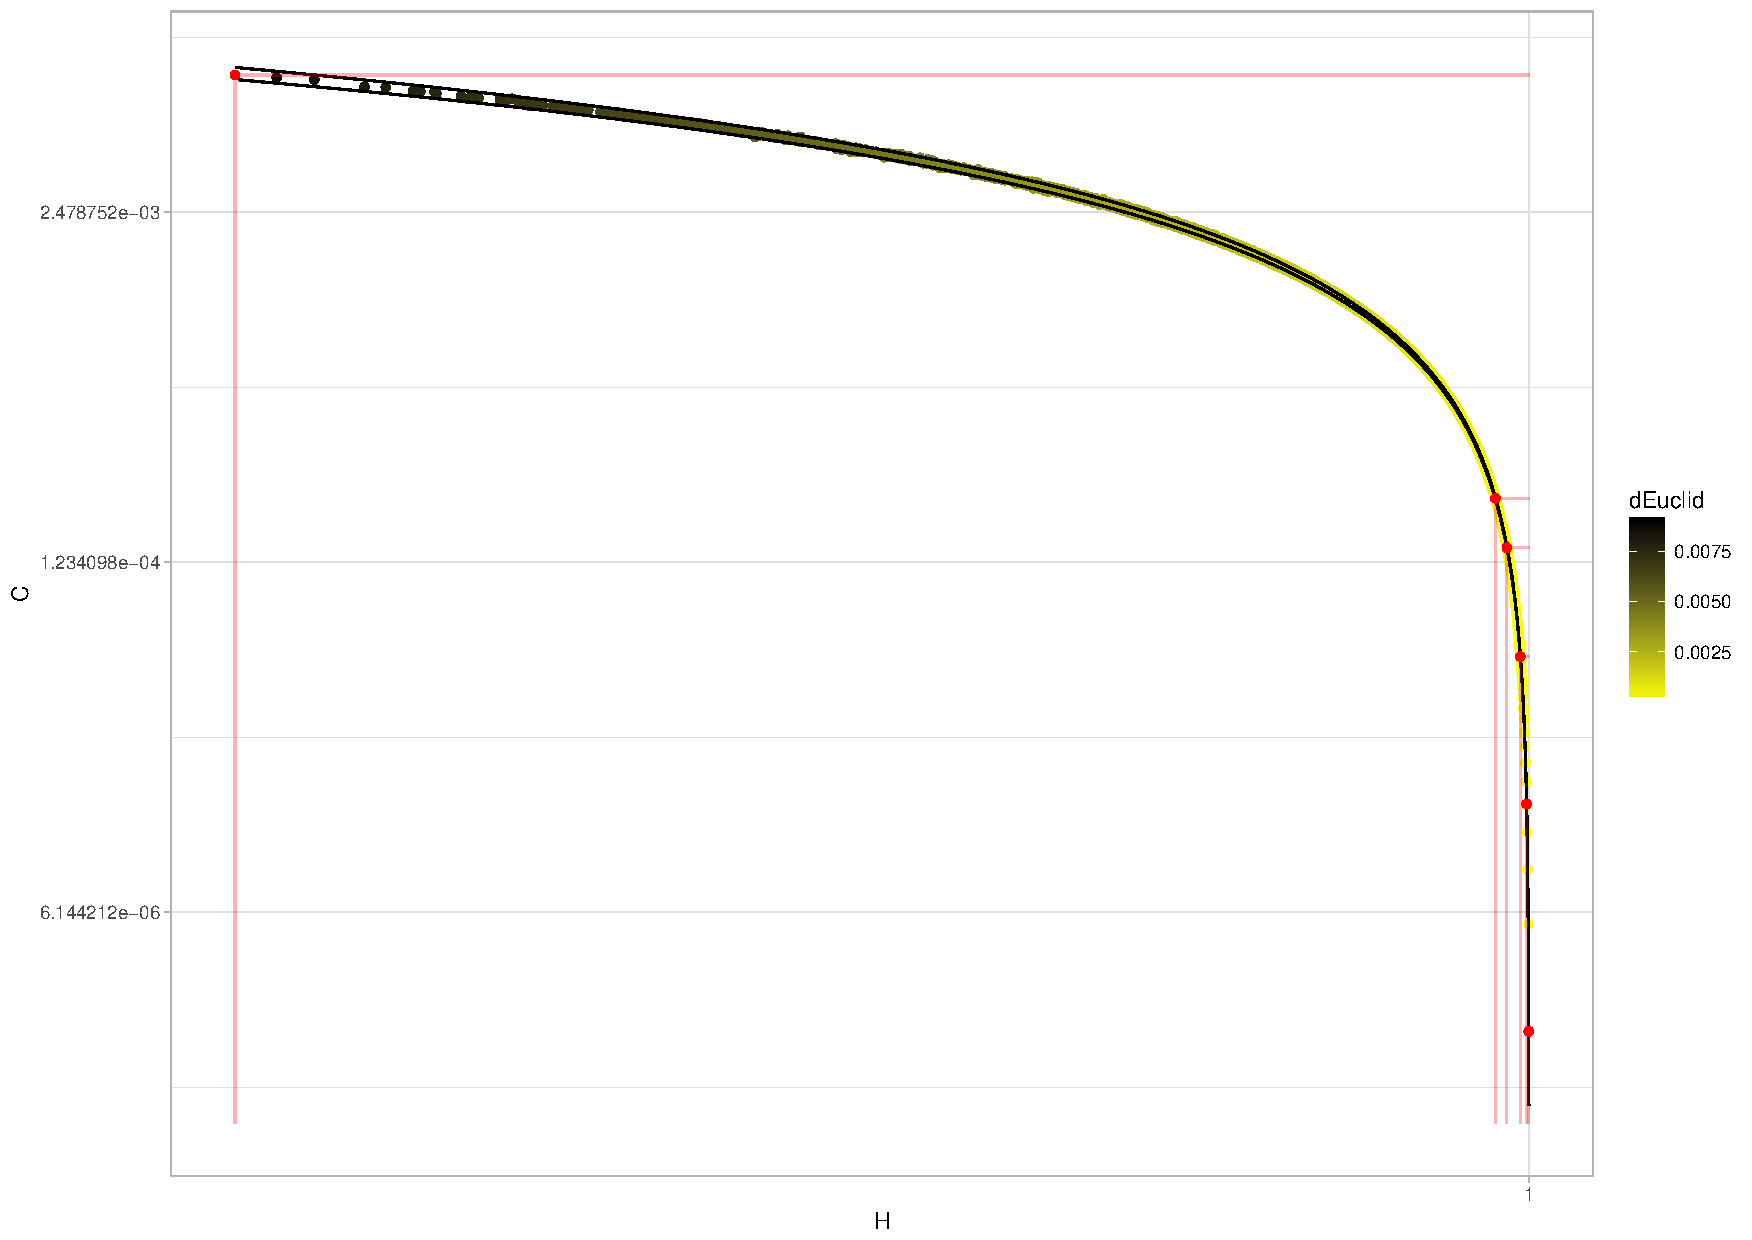
\includegraphics[width=.48\linewidth]{ScatterQuantD3tau1log}}
\caption{Diagramas de dispersão das sequências quânticas para o caso $D=3$ e $\tau=1$.}\label{Fig:QuantD3tau1}
\end{figure}

\begin{figure}
\centering
\subfigure[Escala linear\label{Fig:ScatterQuantD3tau10}]{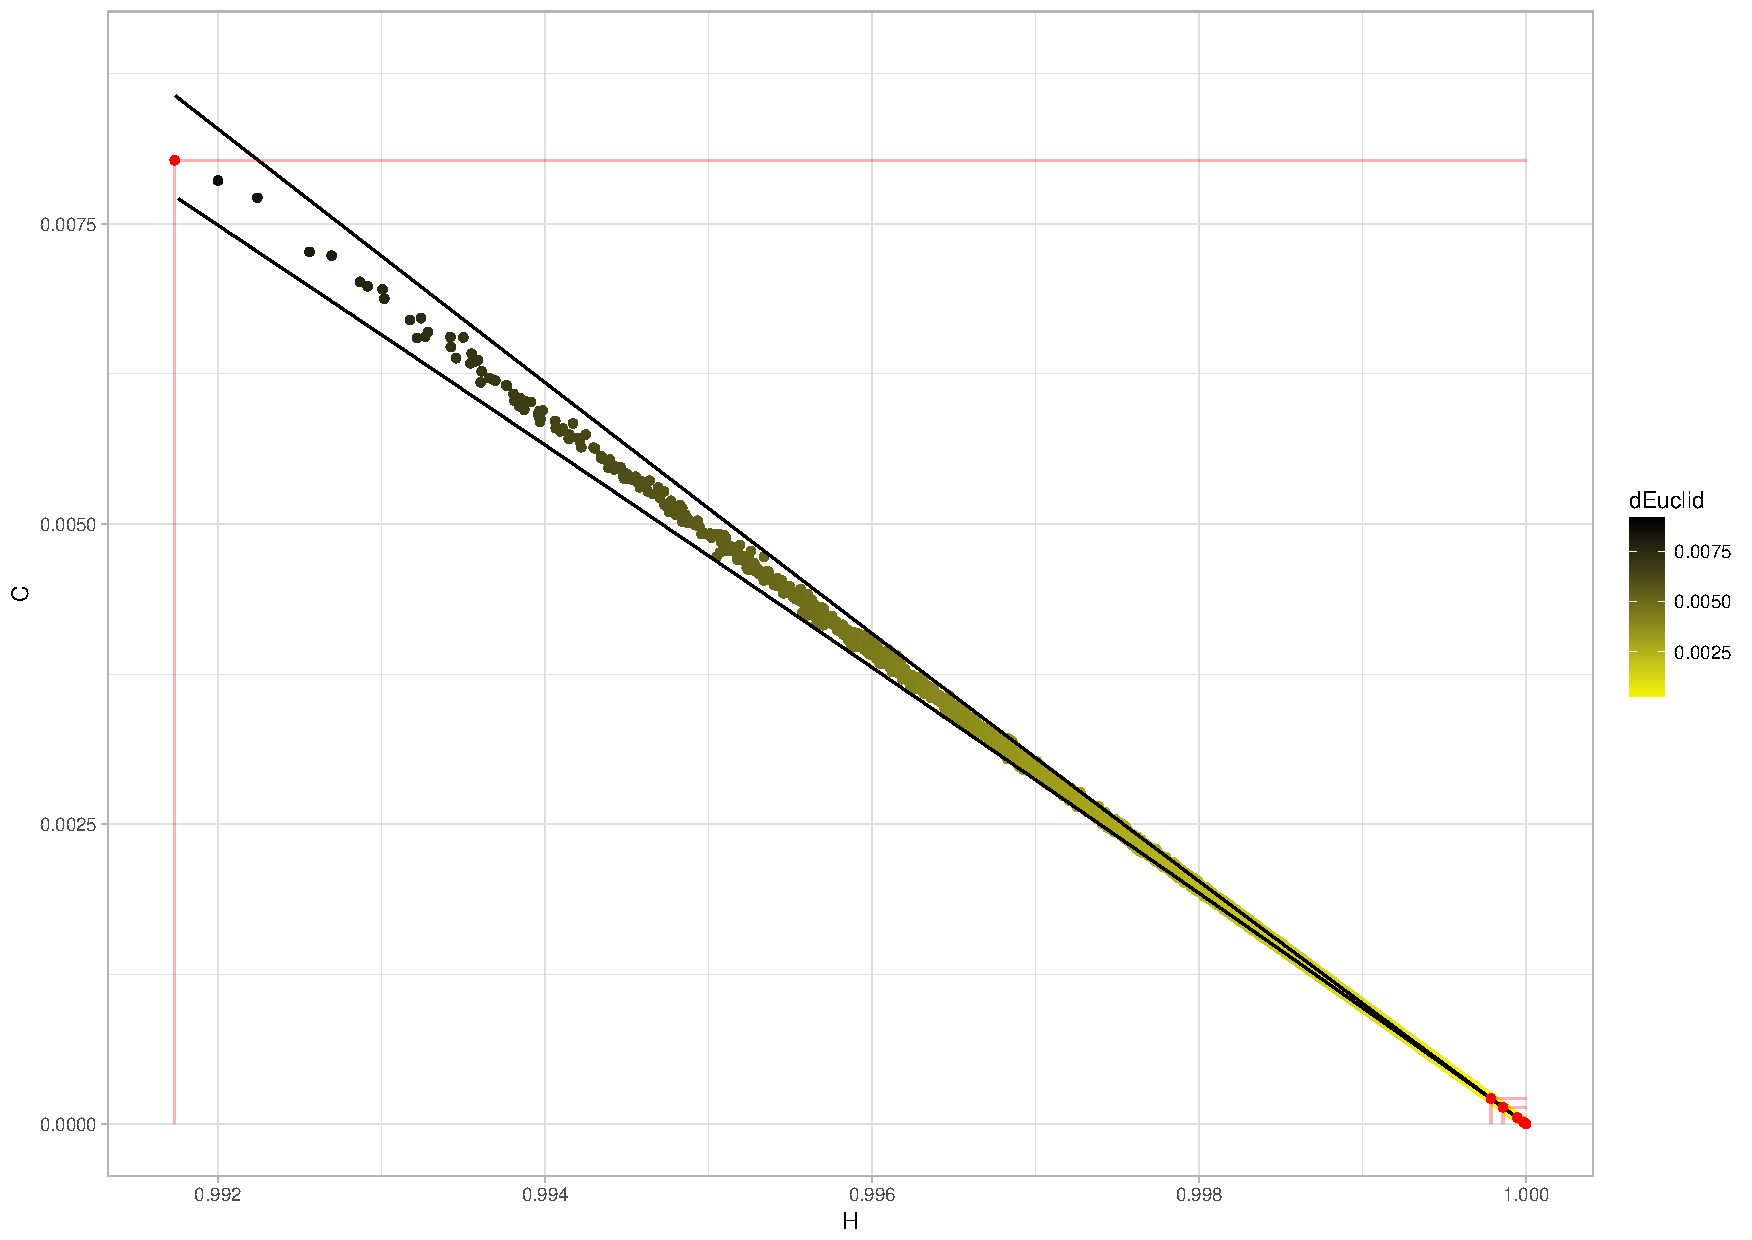
\includegraphics[width=.48\linewidth]{ScatterQuantD3tau1}}
\subfigure[Escala logarítmica\label{Fig:ScatterQuantD3tau10log}]{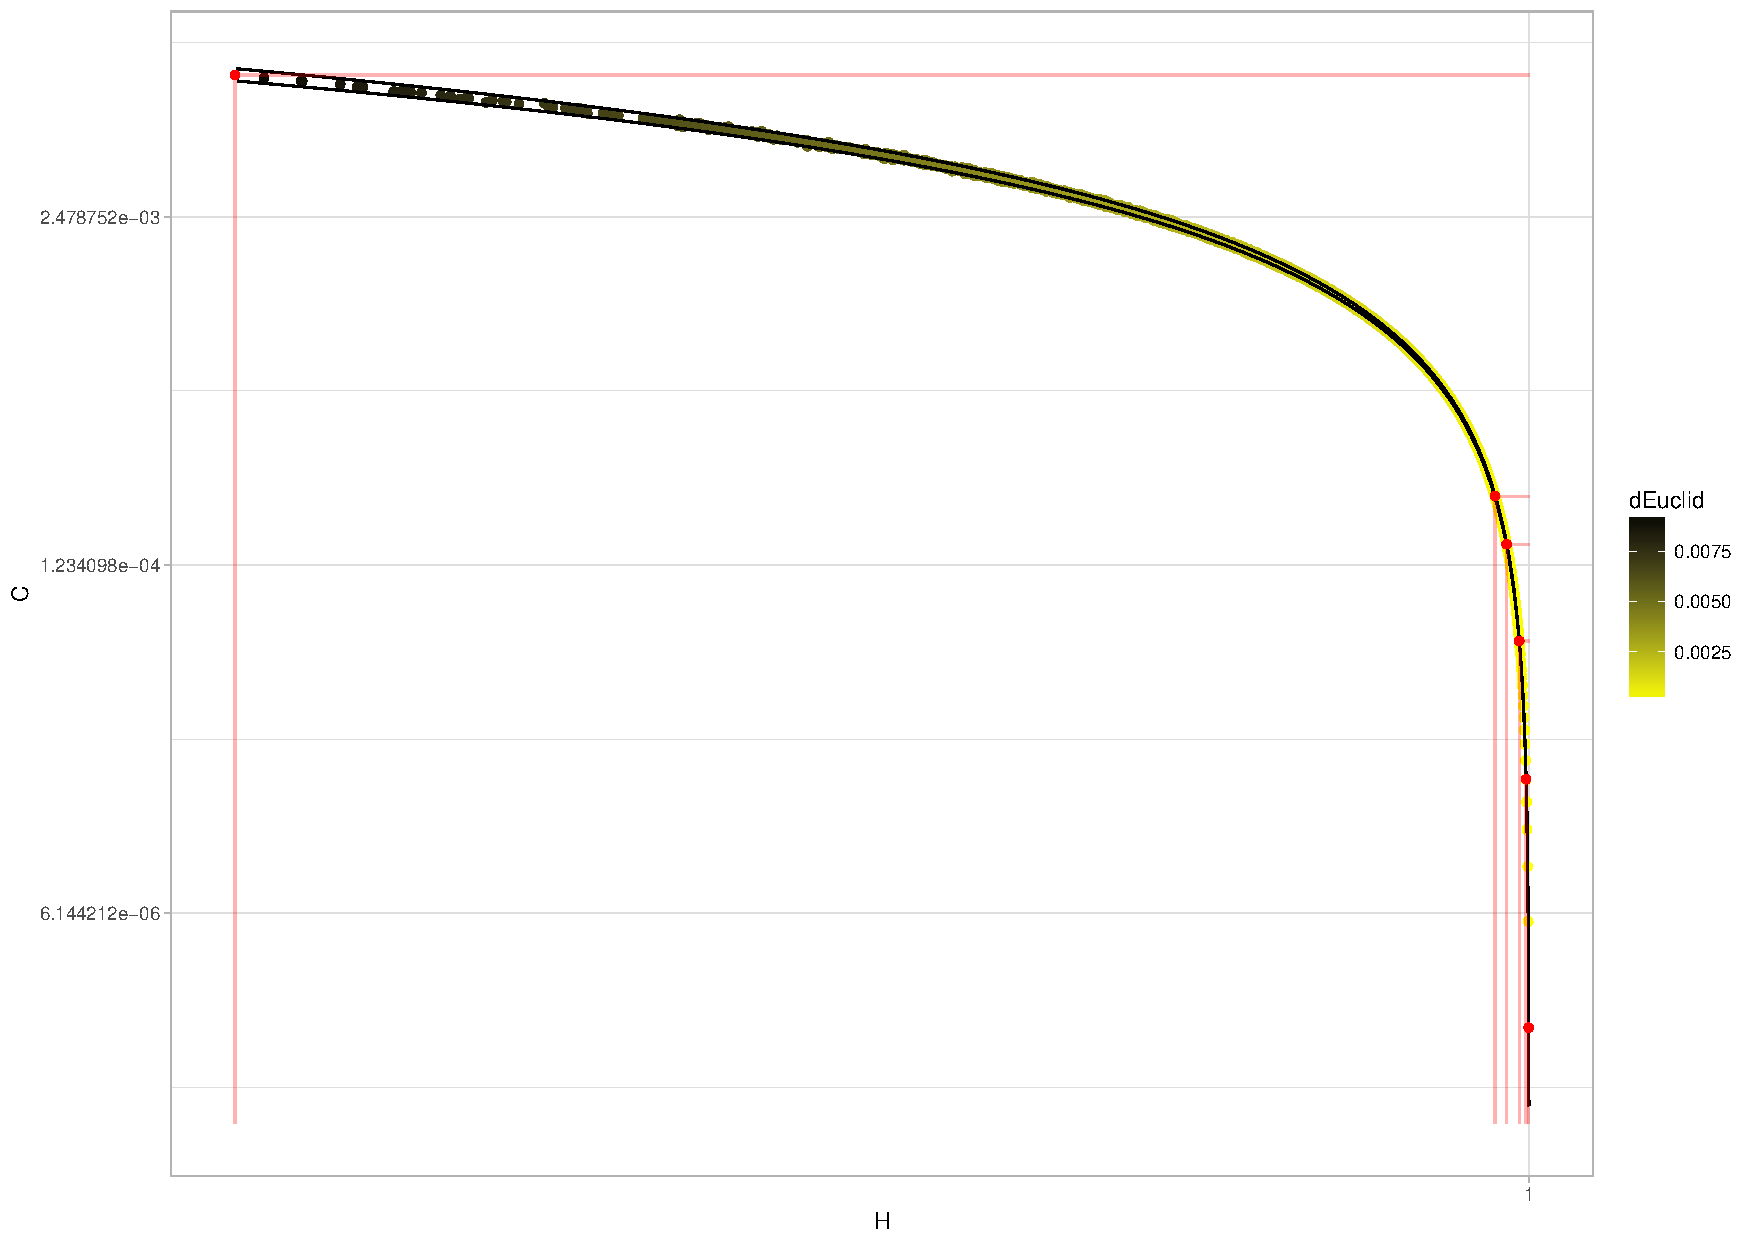
\includegraphics[width=.48\linewidth]{ScatterQuantD3tau10log}}
\caption{Diagramas de dispersão das sequências quânticas para o caso $D=3$ e $\tau=10$.}\label{Fig:QuantD3tau10log}
\end{figure}

\begin{figure}[hbt]
	\centering
	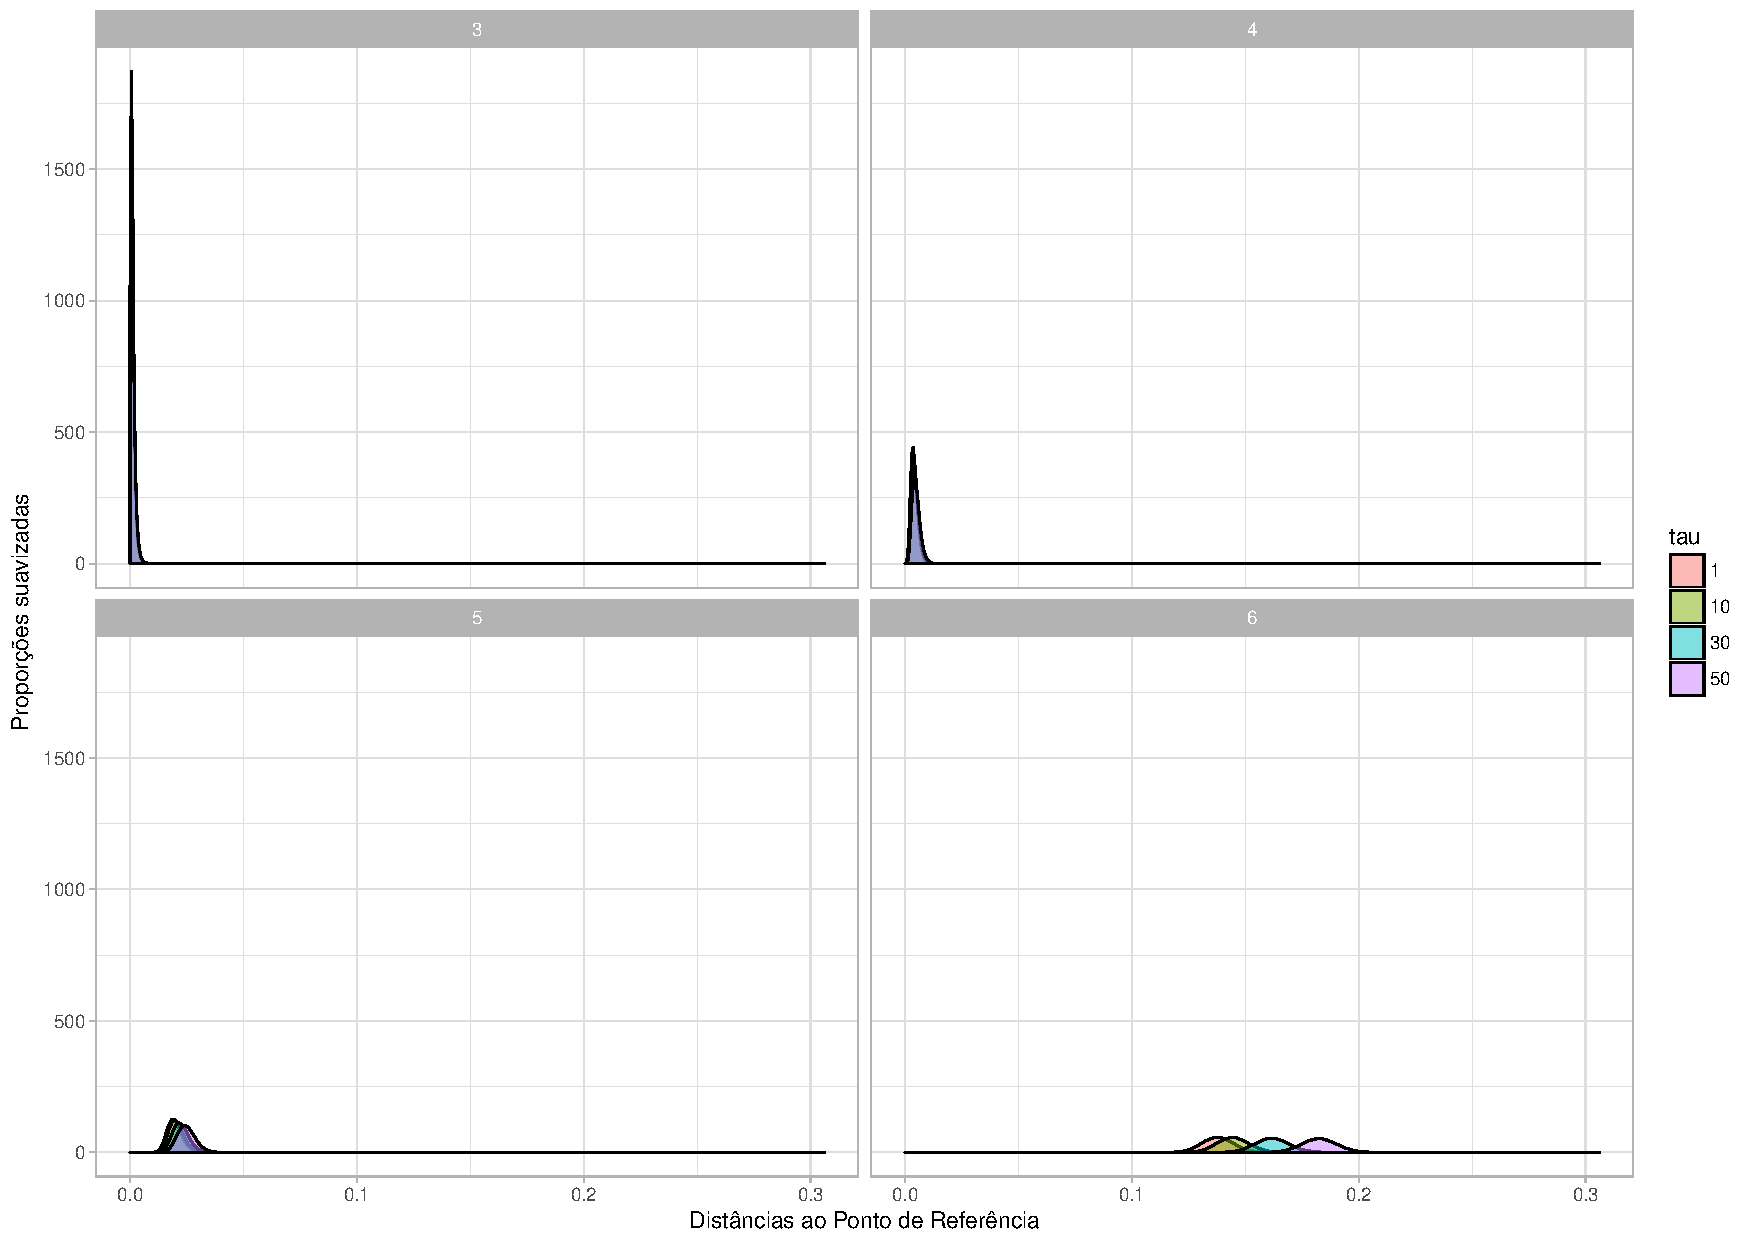
\includegraphics[width=\linewidth]{HistoDistanciasRandTodas}
	\caption{Histogramas suavizados das distâncias euclidianas dos padrões ao ponto de referência, para $D\in\{3,4,5,6\}$ (colunas) e $\tau\in\{1,10,30,50\}$ (linhas).}\label{Fig:HistoDistanciasRandTodas}
\end{figure}



\section{Análise das sequências de rádio}


Antes de analisar os diagramas de dispersão, analisaremos a distribuição empírica das distâncias ao ponto de referência.

A figura~\ref{Fig:HistoDistanciasRandTodas} sugere que o comportamento das distâncias euclidianas ao ponto de referência muda conforme o tamanho do padrão $D$ varia.
Além disso, também são perceptíveis mudanças de comportamento em funçao do \textit{lag} $\tau$ quando $D=5,6$.

No que segue analisaremos o comportamento dessas distâncias em detalhes.


\begin{figure}
	\centering
	%\subfigure[Escala linear\label{Fig:ScatterRandD3tau1}]{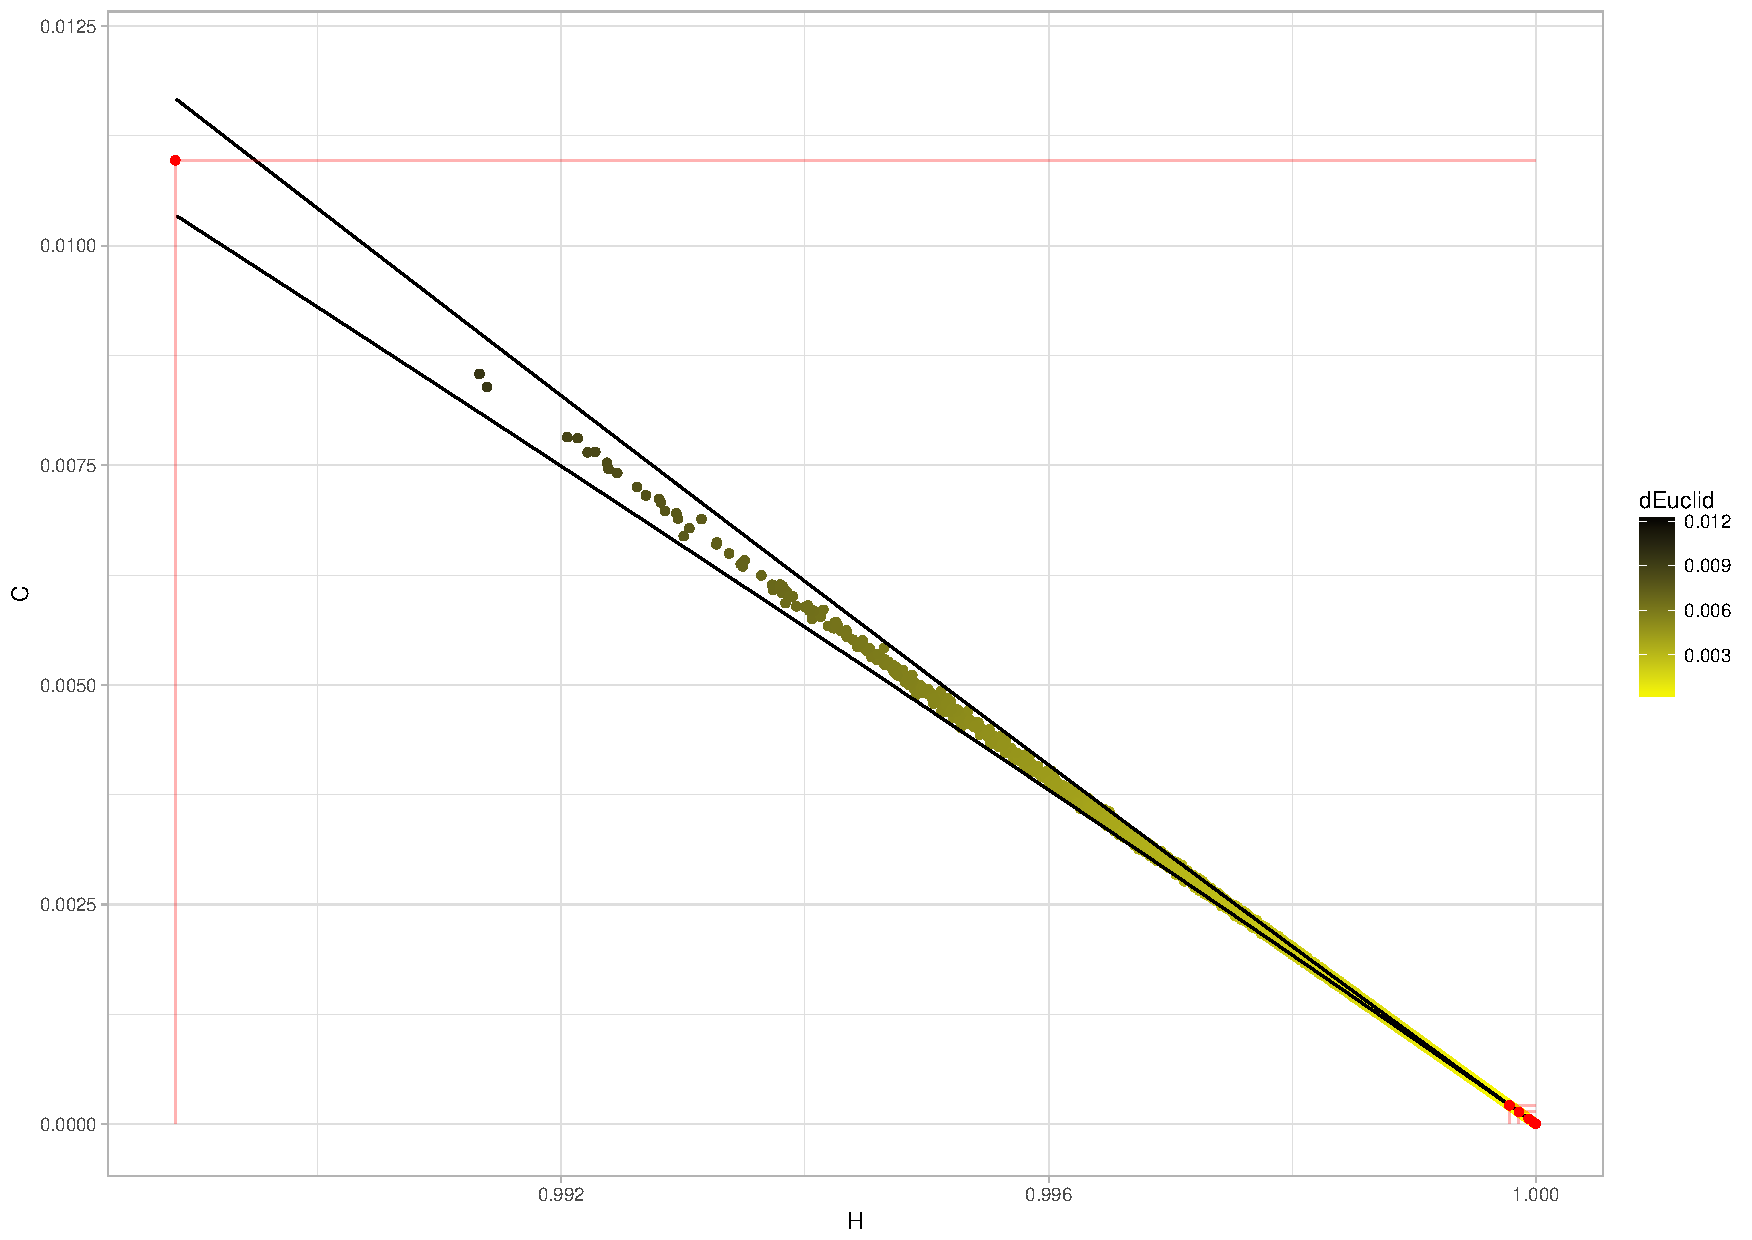
\includegraphics[width=.48\linewidth]{ScatterRandD3tau1}}
	\subfigure[Escala logarítmica\label{Fig:ScatterRandD3tau1log}]{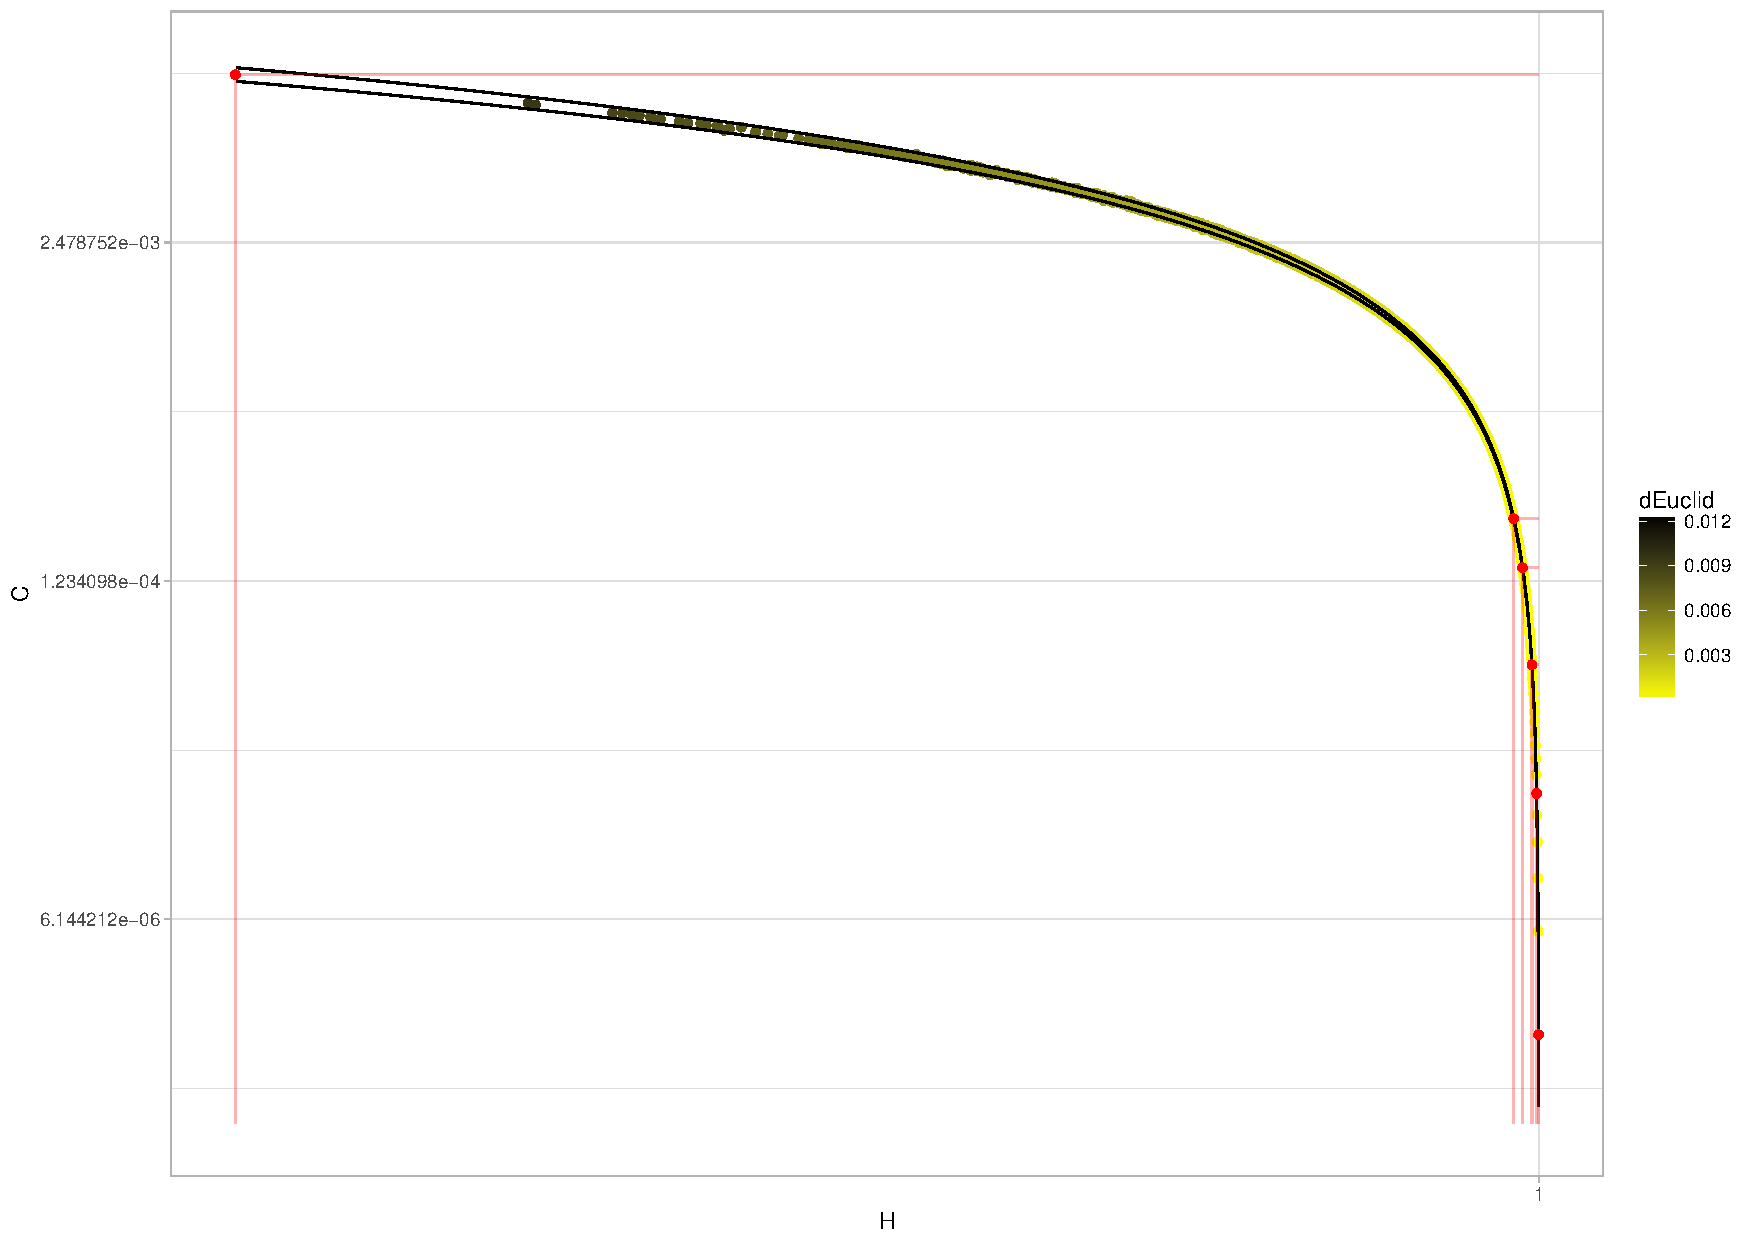
\includegraphics[width=.48\linewidth]{ScatterRandD3tau1log}}
	\caption{Diagramas de dispersão das sequências de rádio para o caso $D=3$ e $\tau=1$.}\label{Fig:RadioD3tau1}
\end{figure}

\begin{figure}
	\centering
%	\subfigure[Escala linear\label{Fig:ScatterRandD3tau10}]{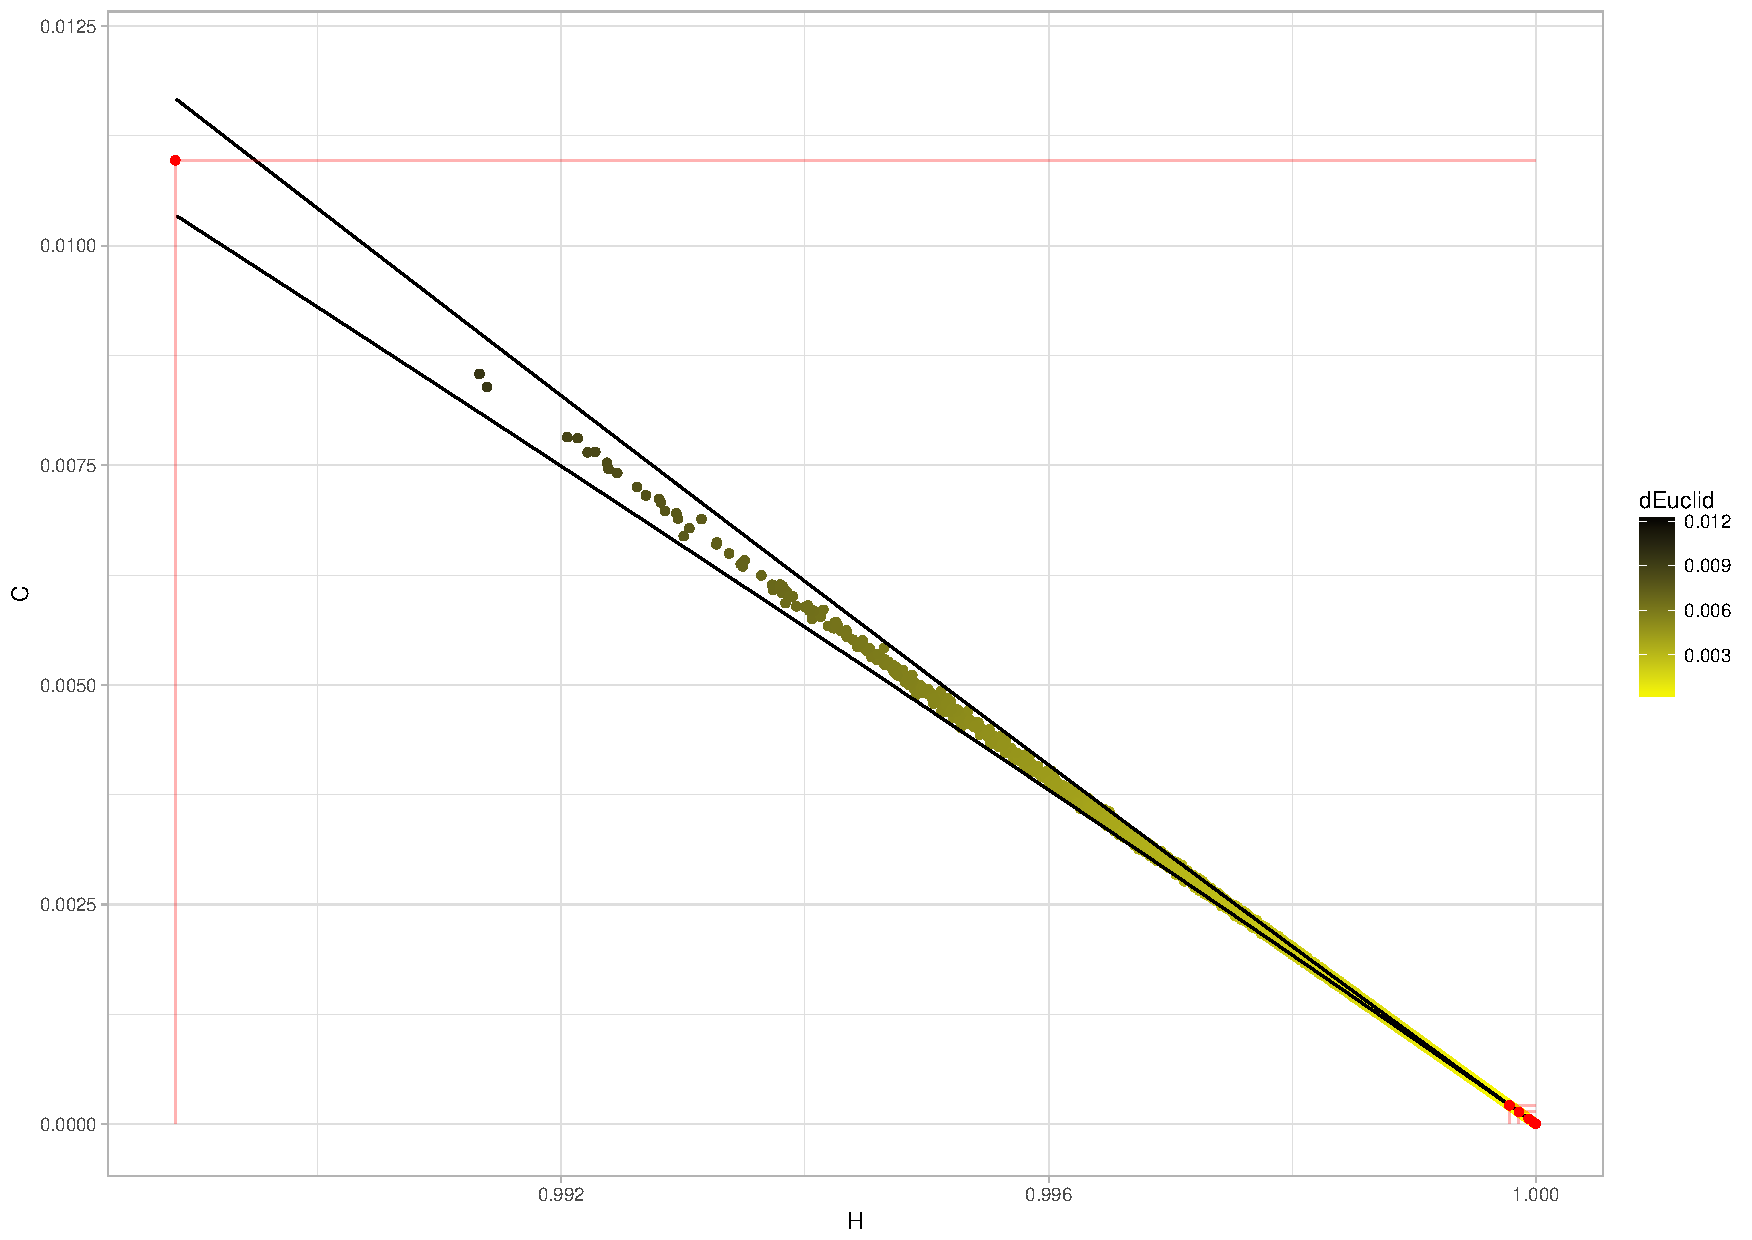
\includegraphics[width=.48\linewidth]{ScatterRandD3tau1}}
	\subfigure[Escala logarítmica\label{Fig:ScatterRandD3tau10log}]{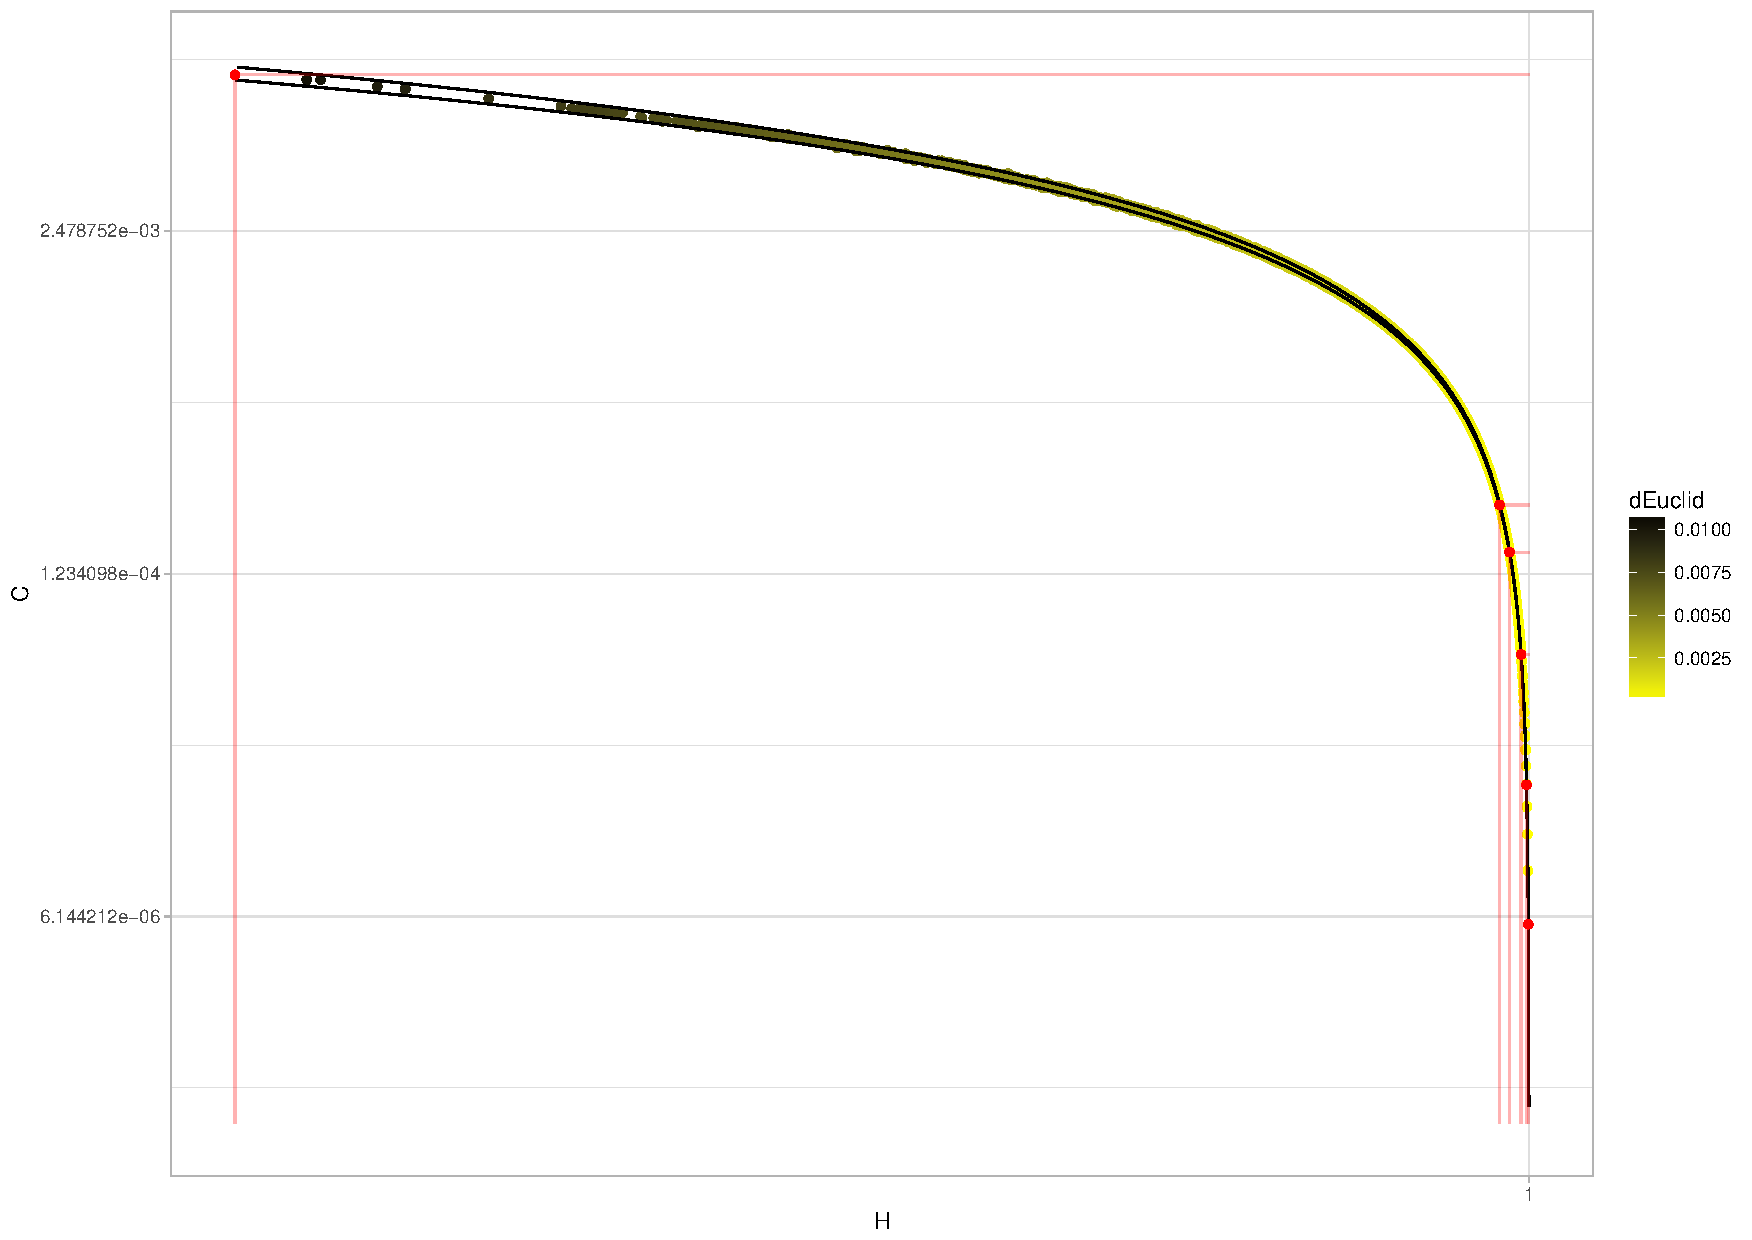
\includegraphics[width=.48\linewidth]{ScatterRandD3tau10log}}
	\caption{Diagramas de dispersão das sequências quânticas para o caso $D=3$ e $\tau=10$.}\label{Fig:QuantD3tau10}
\end{figure}


\section{Análise das sequências Mersenne-Twister}

\begin{figure}
	\centering
	%	\subfigure[Escala linear\label{Fig:ScatterRandD3tau10}]{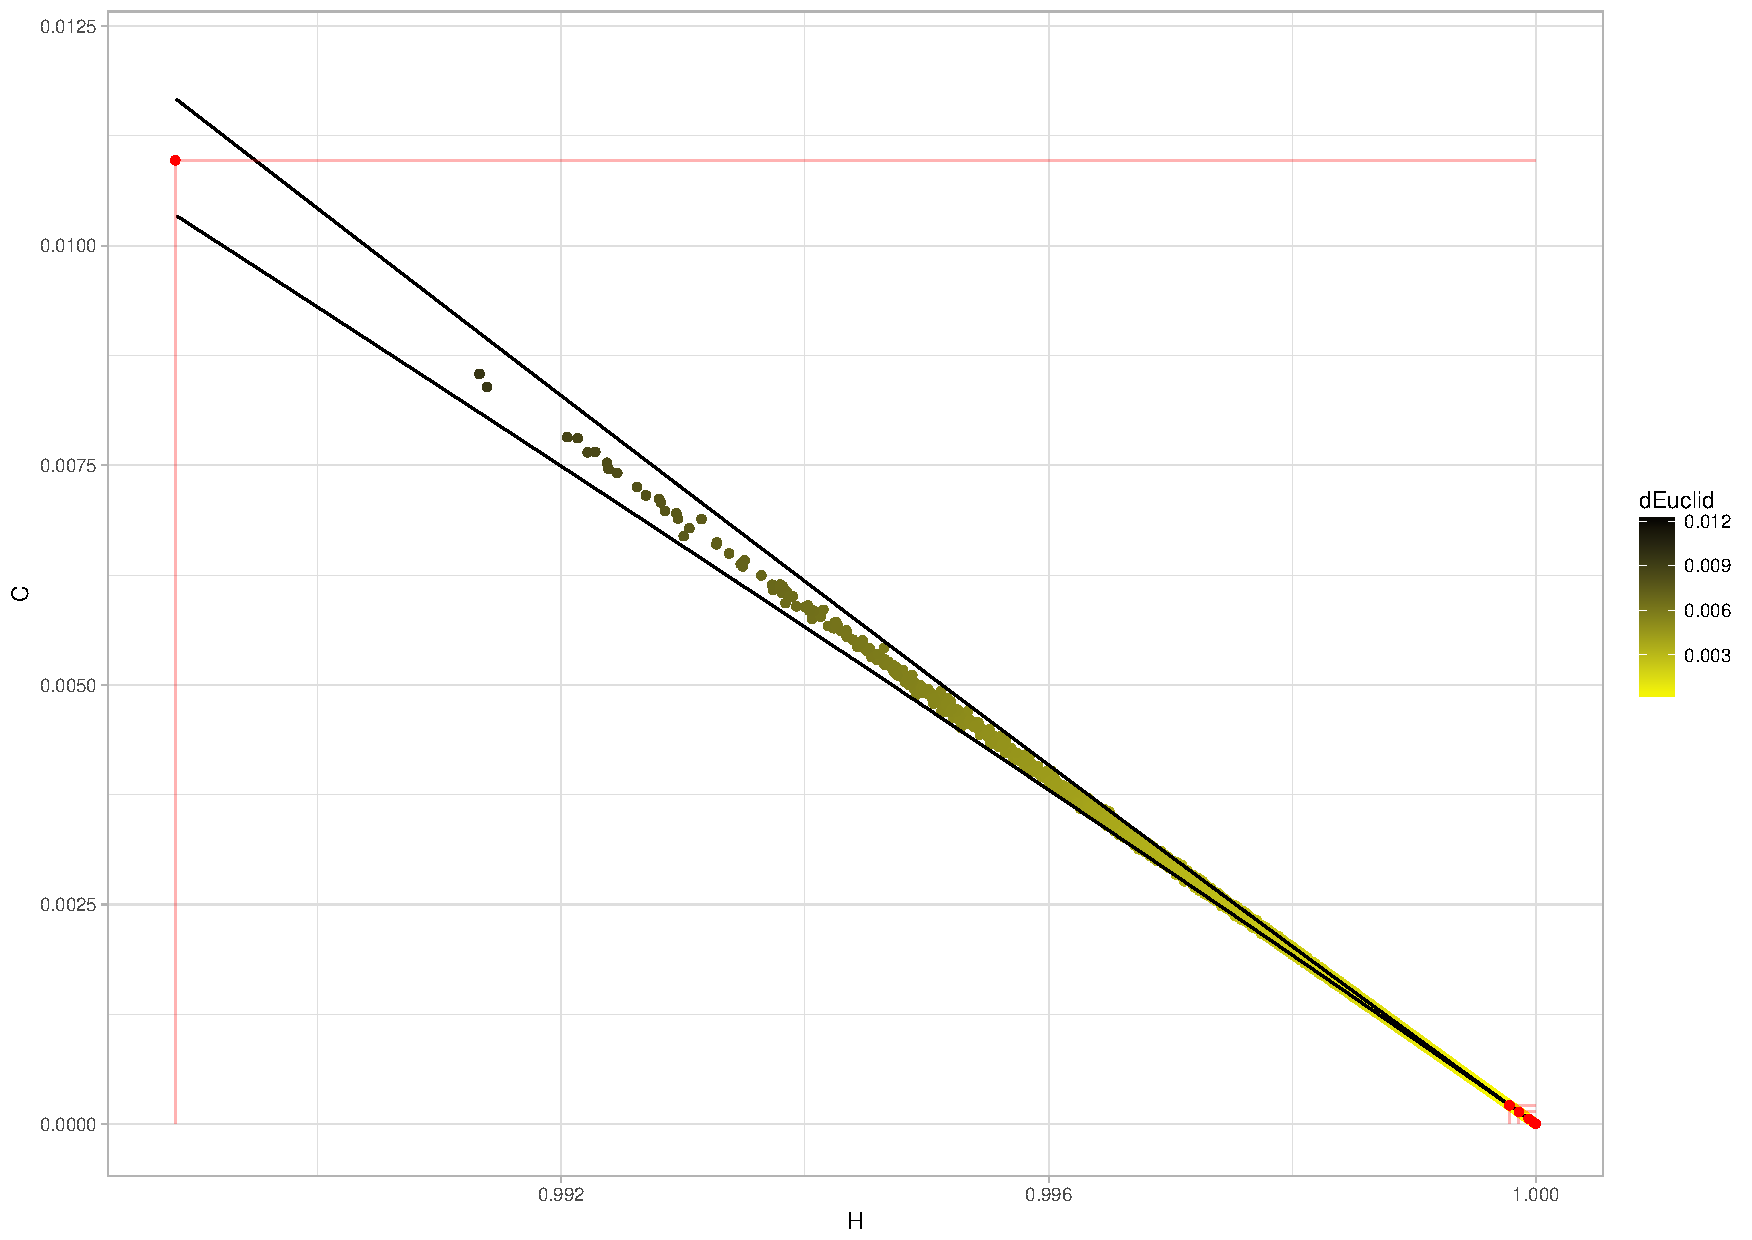
\includegraphics[width=.48\linewidth]{ScatterRandD3tau1}}
	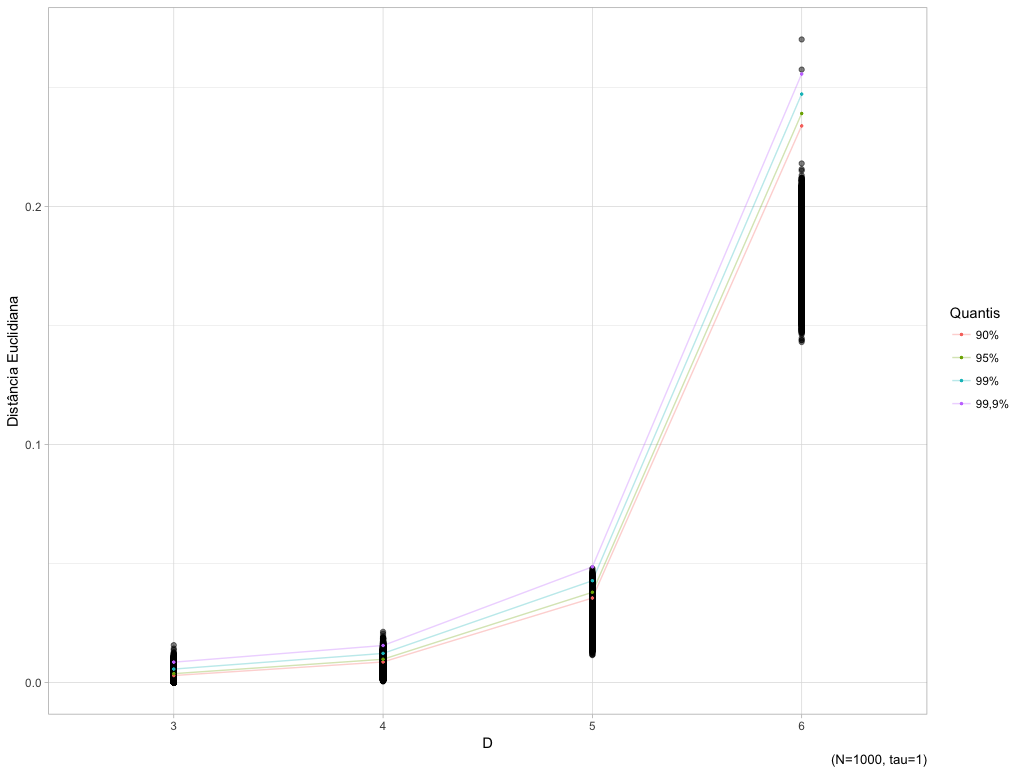
\includegraphics[width=.8\linewidth]{Conf_Int_1k_T1}
	\caption{Intervalos de confiança para o caso $N=1000$ e $\tau=1$.}\label{Fig:Conf_Int_1k_T1}
\end{figure}

\begin{center}
	\fbox{
	\colorbox[RGB]{227, 227, 227}{
	\parbox[t]{.8\linewidth}
		{Neste capítulo tratamos os resultados esperados com a realização do trabalho enquanto que no próximo faremos a conclusão alcançada com o mesmo.}} }
\end{center}

